% !TEX root = ../thesis-example.tex
%
%\chapter{Cosmological Measurements from Angular Power Spectra analysis of BOSS DR12 Tomography}
\chapter{Cosmological Measurements from Angular Power Spectra Analysis of BOSS DR12 Tomography}
\label{Chap:BOSS-Cosmo}

\cleanchapterquote{The truth knocks on the door and you say, "Go away, I'm looking for the truth," and so it goes away. Puzzling.}{Robert M. Pirsig}{(Zen and the Art of Motorcycle Maintenance)}
\vspace*{\fill}

In this chapter, I constrain cosmological parameters by analysing the angular power spectra of the Baryon Oscillation Spectroscopic Survey DR12 galaxies. Sanity and consistency checks are performed in the analysis pipelines, the data-vector and covariances, and in the data itself. Cosmological constraints obtained from these measurements were combined with constraints from Planck CMB experiment as well as the JLA supernovae compilation. Considering a $w$CDM cosmological model measured on scales up to $k_{max} = 0.07h$ Mpc$^{-1}$, I constrain a constant dark energy equation-of-state with a $\sim 4\%$ error at the 1-$\sigma$ level: $w_0 = -0.993^{+0.046}_{-0.043}$, together with $\Omega_m = 0.330\pm 0.012$, $\Omega_b = 0.0505 \pm 0.002$, $S_8 \equiv \sigma_8 \sqrt{\Omega_m/0.3} = 0.863 \pm 0.016$, and $h = 0.661 \pm 0.012$. For the same combination of datasets, but now considering a $\Lambda$CDM model with massive neutrinos and the same scale cut, I find: $\Omega_m = 0.328 \pm 0.009$, $\Omega_b = 0.05017^{+0.0009}_{-0.0008}$, $S_8 = 0.862 \pm 0.017$, and $h = 0.663^{+0.006}_{-0.007}$ and a 95\% credible interval (CI) upper limit of $\sum m_{\nu} < 0.14$ eV for a normal hierarchy. These results are competitive if not better than standard analyses with the same dataset, and demonstrate this should be a method of choice for future surveys, opening the door for their full exploitation in cross-correlations probes.

\textit{The work presented in this chapter was presented in \citet{2018LoureiroBOSS}.} 
\newpage
%------------------------------------------------------------------------%
%                        COSMOLOGICAL BANANAS
%------------------------------------------------------------------------%
%\section{Cosmological Analysis}\label{Sec:CosmoBananas}
\section{Introduction}
For over 20 years, the current cosmological paradigm, the $\Lambda$CDM model, is the most intriguing mystery modern cosmologists are collectively trying to solve. For an extremely simple model -- containing only six free parameters -- the current scenario fails to explain the nature of two of the most important characteristics of this scenario: dark energy and cold dark matter. If warm, dark matter could be easily explained by the energy density of cosmic neutrinos; however, since neutrinos, even having non-zero mass, are relativistic the effect they have is the opposite of cold dark matter: they then to wash away structure instead of amplifying the clustering of matter. From the other perspective, the simplest approach to study dark energy is to parametrize it via its equation-of-state parameter, $w_0$. The hopes are that, if measured with sufficient accuracy and precision, $w_0$ could give us hints on what could be the possible nature of such strange component in our Universe. However, if $w_0 = -1$, we continue to fall under the $\Lambda$CDM scenario since dark energy is then better described to be simply the mysterious cosmological constant postulated by \cite{1917Einstein}. State-of-the-art cosmological surveys such as Planck \citep{PlanckCosmology2016,2018PlanckCosmology} and the Dark Energy Survey \citep{2017arXiv170801530D,2018DES-SNe} measure the equation-of-state of dark energy with percent level precision to be that of a cosmological constant case.

\qquad In this Chapter, I present the cosmological implications from the measured angular power spectra of BOSS galaxies (see Chapter \ref{Chap:BOSS}) for flat $\Lambda$CDM, $w$CDM, and a $\Lambda$CDM with $\sum m_{\nu}$ models. Using the theoretical framework and having estimated covariance matrices as described in Section \ref{Sec:Theory}, I performed a Bayesian analysis using the \texttt{PLINY} nested sampler ( \citealt{PlinyRichardThesis} and Rollins et al., \textit{in prep}) and the \textit{Unified Cosmological Library for Parameter Inference} code, or \texttt{UCLPI} (Cuceu et al., \textit{in prep.}). All analyses considered in this section use the auto-power spectra and the cross-power spectra from adjacent tomographic bins -- the measurements presented in Section \ref{Sec:Measurements}. Cross-power spectra between distant bins are not a part of the final BOSS-$C_{\ell}$ data vector.

\qquad I start this Chapter by describing the likelihoods considered for the analysis, then move to advanced consistency checks -- testing cosmological consistency between different redshift bins, different samples and the whole data analysis pipeline. I then present the cosmological constraints for the standard model of cosmology, $\Lambda$CDM; its extension, $w$CDM; and $\Lambda$CDM with massive neutrinos. Together, I present the marginalised 1D credible contours and the Bayes factor analysis, and the marginalised 2D credible intervals for the cosmological parameters considered in each model.

%------------------------------------------------------------------------%
%                        	LIKELIHOODS! 
%------------------------------------------------------------------------%
\section{Likelihoods, Priors \& Bayes Factor}\label{Sec:LikelihoodsPriors}

The cosmological analysis performed in this work follows a standard Bayesian analysis framework as commonly performed in the literature, e.g. \cite{Blake2007,Thomas2011,2017MNRAS.465.1454H,2017arXiv170801530D}. 

\qquad The posterior distribution of the cosmological parameters, $\pmb{\Theta}$, given the measured angular power spectra, $\hat{S}_{\Delta\ell}$, and a model $\mathcal{M}$ can be written as a marginalisation of the full posterior over the nuisance parameters, $\pmb{\nu}$:

\EQ{MargPost}{\Pr (\pmb{\Theta}|\hat{S}_{\Delta\ell}, \mathcal{M}) = \int \Pr(\pmb{\Theta}, \pmb{\nu} | \hat{S}_{\Delta\ell}, \mathcal{M})d\pmb{\nu}  }
The full posterior distribution can be written as:

\EQ{FullPost}{
\Pr (\pmb{\Theta}, \pmb{\nu} | \hat{S}_{\Delta\ell}, \mathcal{M}) = \frac{\mathcal{L}(\hat{S}_{\Delta\ell}|\pmb{\Theta}, \pmb{\nu}, \mathcal{M}) \pi(\pmb{\Theta}, \pmb{\nu})}{\mathcal{Z}({\hat{S}_{\Delta\ell}}| \mathcal{M})}
}
where $\mathcal{L}(\hat{S}_{\Delta\ell}|\pmb{\Theta}, \pmb{\nu}, \mathcal{M})$ is the likelihood, $\pi(\pmb{\Theta}, \pmb{\nu})$ is the prior on the sampled parameters, and $Z({\hat{S}_{\Delta\ell}}| \mathcal{M})$ is the evidence, which is calculated using \texttt{PLINY}, a nested sampler used in the analysis (\citealt{PlinyRichardThesis} and Rollins et al., \textit{in prep}; \cite{2008FerozHobson}).


\qquad If one had access to the true covariance matrix $\Sigma$, the log likelihood, assumed here to be Gaussian, would be:
\begin{align}
\mathcal{L_G}(\hat{S}_{\Delta\ell}|\pmb{\Theta}, \pmb{\nu}) = & \frac{1}{\sqrt[]{\vert 2\pi \Sigma \vert}} \exp\bigg\{ - \frac{1}{2} \big[ \hat{S}_{\Delta\ell} - S^{th}_{\Delta\ell}(\pmb{\Theta}, \pmb{\nu})\big]^T \Sigma^{-1} \big[ \hat{S}_{\Delta\ell} - S^{th}_{\Delta\ell}(\pmb{\Theta}, \pmb{\nu})\big]\bigg\}
\label{Eq:GaussianLike}
\end{align}
where $S^{th}_{\Delta\ell}(\pmb{\Theta}, \pmb{\nu})$ is the theoretical angular power spectra after being convolved with the mixing matrix (Eq. \eqref{Eq:Cl_Conv}) and binned into the same bandwidths as the data (Eq. \eqref{Eq:S_delta_ell2}). I omitted the  dependency on $\mathcal{M}$ on Eq. \eqref{Eq:GaussianLike} as it is not relevant.

\qquad However, this is not the case when estimating the covariance matrix $\mathcal{C}$ from simulations (Equation \ref{Eq:Covariance}). Even though $\mathcal{C}$ can be an unbiased estimator of the true covariance $\Sigma$, its inverse $\mathcal{C}^{-1}$ is not necessarily an unbiased estimator of the inverse covariance $\Sigma^{-1}$, needed to estimate the likelihood in Equation \eqref{Eq:GaussianLike}. \cite{Hartlap2007} proposed to keep using the Gaussian likelihood, and to apply a simple rescaling to the inverse of the estimated covariance matrix in order to de-bias it \citep{AndersonBook}.

\begin{equation}
\Sigma^{-1} \rightarrow \alpha \mathcal{C}^{-1}
\end{equation}
where 

\begin{equation}
\alpha = \frac{N_s - p - 2}{N_s - 1}
\end{equation}
and $N_s$ is the number of simulations and $p$ is the size of the data vector. 

\qquad More recently, \cite{2016SellentinHeavens} (hereafter, SH16) showed that when replacing the true covariance $\Sigma$ with an estimated $\mathcal{C}$, one should marginalise over the true covariance conditioned on the estimated one from simulations.  The resulting likelihood is no longer Gaussian; instead, the likelihood is now given by a multivariate t-distribution (SH16):

\begin{equation}
\mathcal{L_{SH}}(\hat{S}_{\Delta\ell}|\pmb{\Theta}, \pmb{\nu}) = \frac{\overline{c}_p}{\vert \mathcal{C} \vert^{1/2}} \Big[1 + \frac{(\hat{S}_{\Delta\ell} - S^{th}_{\Delta\ell})^T \mathcal{C}^{-1} (\hat{S}_{\Delta\ell} - S^{th}_{\Delta\ell})}{N_s + 1}\Big]^{\frac{-N_s}{2}}
\end{equation}
where
\begin{equation}
\overline{c}_p = \frac{\Gamma\big(\frac{N_s}{2}\big)}{\big[\pi(N_s - 1)\big]^{p/2} \Gamma\big(\frac{N_s - p}{2}\big)}
\end{equation}
and $\Gamma$ is the gamma function.

\begin{table}
\centering
\caption[Maximum multipole considered in the cosmological analysis for each tomographic redshift bin.]{Maximum multipole considered in the cosmological analysis for each tomographic redshift bin. All the samples start at $\ell_{min} = 13.5$ and have a bandwidth of $\Delta\ell = 8$. When considering the cross-power spectra between bins, the lower $\ell_{max}$ is used. The $\ell_{max}^{5\%}$ column corresponds to a $k_{max}  \lesssim 0.07 h$ Mpc$^{-1}$, and the $\ell_{max}^{10\%}$ column corresponds to a  $k_{max}  \lesssim 0.10 h$ Mpc$^{-1}$.}
\label{Tb:EllCuts}
\begin{tabular}{lllll}
\hline
\hline
Sample Bin & $z_{min}$ & $z_{max}$ & $\ell_{max}^{5\%}$ & $\ell_{max}^{10\%}$\\
\hline
\hline
LOWZ--0  & 0.15      & 0.20      & 53	&	69 \\
LOWZ--1  & 0.20      & 0.25      & 77	&	93 \\
LOWZ--2  & 0.25      & 0.30      & 93	&	109\\
LOWZ--3  & 0.30      & 0.35      & 109	&	133\\
LOWZ--4  & 0.35      & 0.40      & 125	&	157\\
LOWZ--5  & 0.40      & 0.45      & 141	&	173\\
CMASS--6 & 0.45      & 0.50      & 157	&	221\\
CMASS--7 & 0.50      & 0.55      & 165	&	237\\
CMASS--8 & 0.55      & 0.60      & 189	&	261\\
CMASS--9 & 0.60      & 0.65      & 197	&	277\\
CMASS--10 & 0.65      & 0.70      & 213	&	317\\
CMASS--11 & 0.70      & 0.75      & 245	&	333\\
CMASS--12 & 0.75      & 0.80      & 261	&	381\\
\hline
\hline
\end{tabular}
\end{table}

\qquad Even though the non-linear model described in Section \ref{Sec:NonLin} is sufficiently reliable, I performed cuts in $\ell_{max}$ for each of the tomographic redshift bins in order to exclude non-linear scales. In order to make this choice, I used a fiducial cosmology (the same used in Section \ref{Sec:ConsistControl}) to generate theory $C_{\ell}$s and performed a preliminary cut in $\ell_{max}$ where the percent deviation between the linear and non-linear models were smaller than $5\%$. I performed robustness checks on the $5\%$ deviation cut choice by extending the cuts to $\ell_{max}$ which had a deviation up to $20\%$ and concluded that my cosmological results could be trusted up to a $15\%$ deviation between linear and non-linear theories for this fiducial test. In this work I present results where this percentage cut is $5\%$ and $10\%$. For avoidance of doubt, for the fiducial cosmology of choice, applying a $5\%$ implies rejecting the majority of modes $k \lesssim 0.07 h$ Mpc $^{-1}$, whereas $10\%$ implies rejecting the majority of modes $k \lesssim 0.1 h$ Mpc $^{-1}$. The resulting cuts can be found in table \ref{Tb:EllCuts}. As for the $\ell$ cuts for cross-power spectra, I chose the lowest $\ell_{max}$ between the two relevant bins in order to keep a consistent and conservative cut for each bin.

\qquad I used a total of 28 nuisance parameters ($\pmb{\nu}$) in the BOSS $C_{\ell}$ likelihood analysis in most of the results for a $5\%$ cut on $\ell_{max}$. These parameters are: a scale independent bias, $b(z)$, for each redshift bin; a redshift error dispersion, $\sigma_s(z)$ (Equation \ref{Eq:GaussianErrNz}), for each redshift bin that takes into account spectroscopic redshift error and Fingers-of-God effects due to shell-crossing (see Section \ref{Sec:SpecNz} for details); and an extra shot-noise term for bins 11 and 12 that is forward modelled into the theoretical angular power spectrum inside the likelihood as:

\EQ{Eq:ExtraNoise}{\hat{S}^{th}_{\Delta\ell} \rightarrow \hat{S}^{th}_{\Delta\ell} + \mathcal{N}}
where $\mathcal{N}$ is a constant that takes into account extra shot-noise due to the very low number of galaxy in these two redshift bins. In the case of a $10\%$ I used two further shot-noise nuisance parameters for bins 9 and 10 respectively as it goes further into the non linear regime where the shot-noise in those bins dominates over the signal.

\qquad I chose flat priors in all Bayesian analysis. These were based on priors used in \cite{JLAdata,2016BOSSCosmology,PlanckCosmology2016,2017arXiv170801530D} and were set equally for all analyses. The prior ranges can be found in table \ref{Tb:Priors} for all parameters considered in the cosmological analysis in this section: the baryonic matter density ($\Omega_b$), the cold dark matter density ($\Omega_{cdm}$), the amplitude of the primordial power spectrum ($A_s$), the spectral index ($n_s$), the Hubble constant ($h$), the equation-of-state of dark energy ($w_0$), the sum of neutrino mass species ($\sum m_{\nu}$), the optical depth at reionisation epoch ($\tau_{reio}$), the bias of BOSS galaxies as a function of redshift ($b(z)$), the redshift dispersion parameter for BOSS galaxies ($\sigma_s(z)$), the extra shot-noise for BOSS galaxies ($\mathcal{N}_i$), the Planck absolute calibration parameter ($y_{cal}^{Planck}$), and the absolute magnitude of SNe Ia at peak light in blue band ($M_B^{JLA}$).

\begin{table}
  \centering
  \caption[Prior ranges used in the BOSS analysis.]{Ranges on the flat priors used in all Bayesian analysis. Parameters are divided into two groups: cosmological and nuisance.}
  \label{Tb:Priors}
  \begin{tabular}{cc}
    \hline
    \hline
    Parameter & Prior Range \\
    \hline
        \hline
     $\Omega_b$ & $1 \times 10^{-3}, \, 0.3$    \\
     $\Omega_{cdm}$ & $0.0, \, 0.8$    \\[0.1cm]
     $\ln 10^{10} A_s$ & $2.0, \, 4.0$    \\
     $n_s$ & $0.87, \, 1.07$    \\
     $h$ & 0.55, 0.91 \\
     $w_0$ & -3, -0.3\\
     $\sum m_{\nu}$ & 0.0, 1.0 eV\\[0.1cm]
     $\tau^{Planck}_{reio}$  & 0.0, 0.8 \\
     \hline
     $b(z)$  & 1.1, 3.3 \\
     $\sigma_s(z)$ & $1 \times 10^{-6}, 9 \times 10^{-3}$ \\
     $\mathcal{N}_{9}, \, \mathcal{N}_{10}$ & $0.0, \, 1\times 10^{-4}$ \\
     $\mathcal{N}_{11}$ & $0.0, \, 8\times 10^{-5}$ \\
     $\mathcal{N}_{12}$ & $0.0, \, 4\times 10^{-4}$ \\
     $y_{cal}^{Planck}$ & $0.99, \, 1.01$ \\
     $M_B^{JLA}$ & -20.0,\, -18.5.\\
     \hline
        \hline
  \end{tabular}
\end{table}

\qquad Finally, to perform consistency checks between BOSS DR12 and the external datasets described in Section \ref{Sec:ExternalData}, I use the Bayes factor. The Bayes factor for the consistency of two datasets (A and B) is given by:

\begin{equation}
R_{A,B} = \frac{\mathcal{Z}(\vec{A},\vec{B}|M)}{\mathcal{Z}(\vec{A}|M)\mathcal{Z}(\vec{B}|M)}
\label{Eq:BayesFactor}
\end{equation}
\noindent or, for three datasets (A, B, and C):

\begin{equation}
R_{A,B,C} = \frac{\mathcal{Z}(\vec{A},\vec{B},\vec{C}|M)}{\mathcal{Z}(\vec{A}|M)\mathcal{Z}(\vec{B}|M)\mathcal{Z}(\vec{C}|M)}
\label{Eq:BayesFactor}
\end{equation}

\noindent where $M$ is the model, $\mathcal{Z}(\vec{A},\vec{B}|M)$ is the evidence when the model is fitted to both datasets simultaneously and $\mathcal{Z}(\vec{A}|M)\mathcal{Z}(\vec{B}|M)$ is the product of the evidences when the model is fitted to each dataset individually. Since \pliny is a nested sampler, all the cosmological estimations lead to values for the evidences of each model, dataset, and combination of datasets.


\begin{figure}
\begin{center}
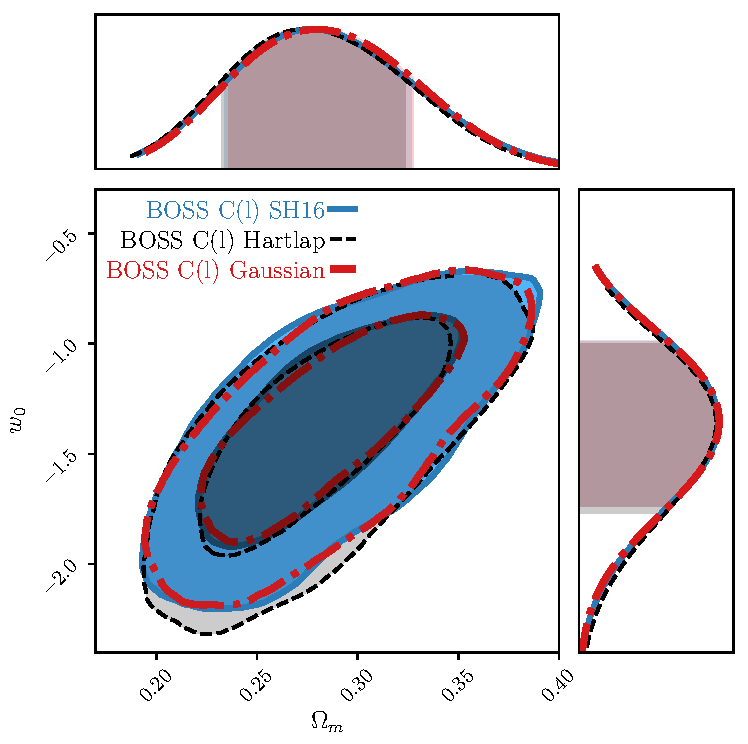
\includegraphics[scale=0.73]{BOSS-FIGS/likelihood_comparisonOmega_cdm_w0.pdf}
\caption[Comparison between the three likelihood methods mentioned in Section \ref{Sec:LikelihoodsPriors} using the BOSS $C_{\ell}$ data only for $\Omega_{m}$ and $w_0$.]{Comparison between the three likelihood methods mentioned in Section \ref{Sec:LikelihoodsPriors} using the BOSS $C_{\ell}$ data only for $\Omega_{m}$ and $w_0$ in a $w$CDM model: Gaussian (red), Gaussian with Hartlap correction (black) and the SH16 (blue) likelihoods. Note how, given the high number of log-normal simulation used to estimate the inverse of the covariance, the Hartlap correction likelihood, SH16, and Gaussian have equivalent contours even though the sampled parameters and likelihood values are different. It is clear from this analysis that the estimated covariance matrix from Section \ref{Sec:Cov} is robust and was estimated with a sufficient number of simulations.}
\label{fig:LikelihoodCompare}
\end{center}
\end{figure}

\qquad In order to perform a robust analysis, the three likelihoods approaches were implemented: Gaussian, Gaussian using the Hartlap correction, and the SH16 t-distribution likelihood. Although the values of the sampled parameters and posterior values were different, the Gaussian + Harlap correction, the SH16, and the Gaussian likelihoods led to very similar cosmological contours. Figure \ref{fig:LikelihoodCompare} shows a comparison between the three likelihood for a $w$CDM
model, using the BOSS $C_{\ell}$'s only, for $w_0$ and $\Omega_m$. In all of the following results in this Section, I use the SH16 likelihood.


%------------------------------------------------------------------------%
%                        	CONSISTENCY CHECKS 
%------------------------------------------------------------------------%
\section{Consistency Checks}
In this section, I perform a series of consistency checks in order to assess the validity of the cosmological parameter estimation pipelines and data samples. 

\subsection{Parameter-dependant Theoretical Covariance Matrix}
\begin{figure}
\begin{center}
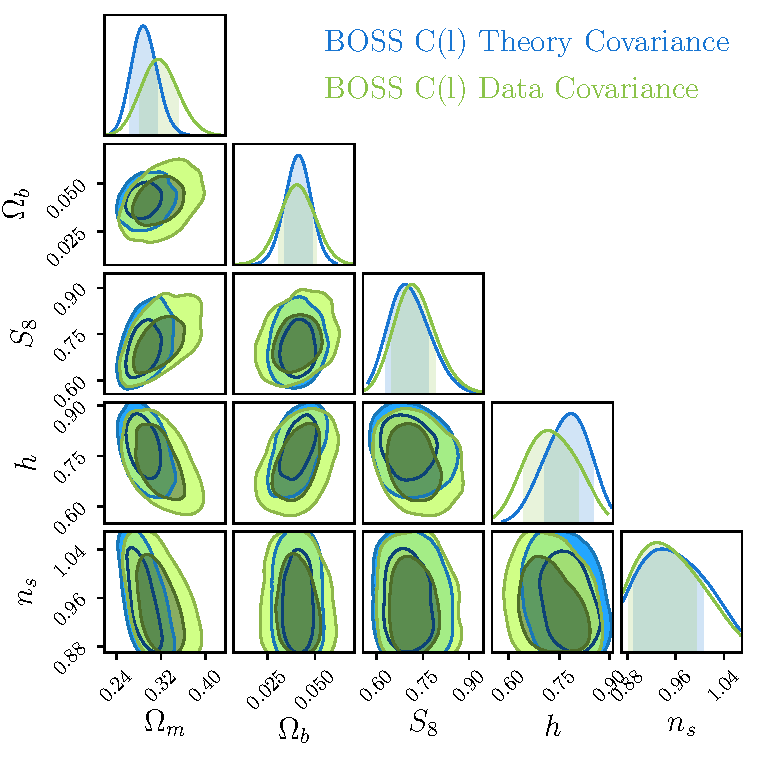
\includegraphics[scale=0.75]{BOSS-FIGS/theoryCovContours.pdf}
\caption[Comparison between $\Lambda$CDM cosmologies recovered using the covariance matrix estimated in Section \ref{Sec:Cov}and the cosmology dependent theoretical covariance matrix from Equation \eqref{Eq:TheoVariance}.]{Comparison between $\Lambda$CDM cosmologies recovered using the covariance matrix estimated in Section \ref{Sec:Cov} (\textit{green contours}, same as the ones from Section \ref{Sec:LCDM}), and the cosmology dependent theoretical covariance matrix from Equation \eqref{Eq:TheoVariance} (\textit{blue contours}). Note that the same parameters were sampled in both cases as the theoretical covariance also depends on the same nuisance parameters. These marginalised credible intervals (CI) 1- and 2-$\sigma$ plots indicate both the estimated covariance matrix and the \uclcl pipeline robustness.}
\label{fig:TheoryCovTriangle}
\end{center}
\end{figure}

An alternative likelihood was implemented in the \uclcl pipeline, based on the theoretical expression I derived for the covariance matrix (Section \ref{Sec:TheoCov}, Equation \eqref{Eq:TheoVariance}) where the signal angular power spectra, $S_{\ell}$, also depends on the sampled parameters. Most standard cosmological analysis in the literature \citep{2016BOSSCosmology,2017arXiv170801530D,2017MNRAS.465.1454H} assume a covariance matrix which is independent of cosmology and which is estimated for a fiducial simulation. Here, I do not expect to obtain the same cosmological contours from this method as those presented in the section that follow; however, I do not expect the contours from this method to disagree significantly with the ones obtained with my estimated covariance matrix. Figure \ref{fig:TheoryCovTriangle} shows the results for this test for a $\Lambda$CDM cosmological model. 

\subsection{Controlled Cosmology Pipeline Test}\label{Sec:ConsistControl}
\begin{figure}
\begin{center}
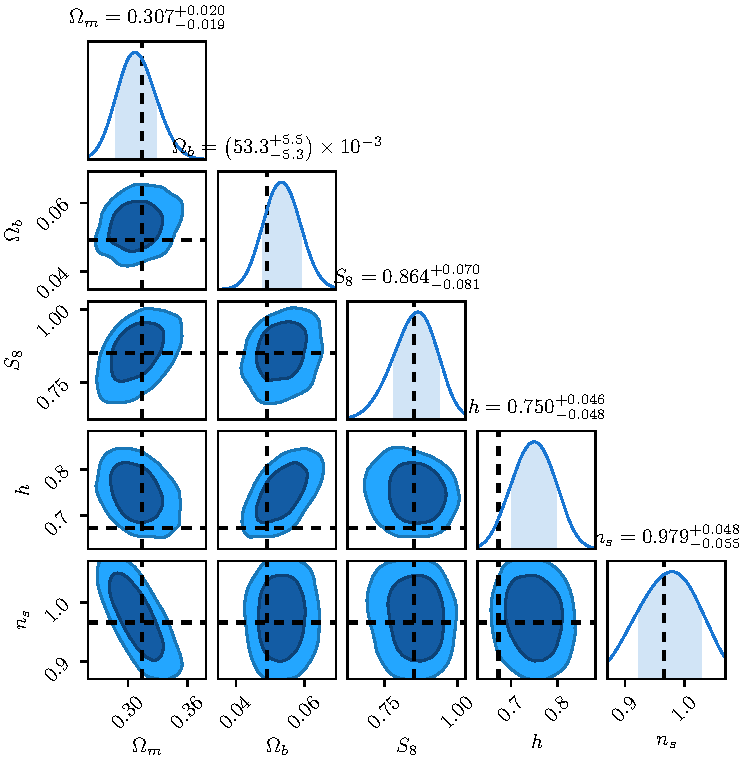
\includegraphics[scale=0.85]{BOSS-FIGS/Controlled_PipelineTest.pdf}
\caption[Cosmological constraints recovered from a controlled cosmology pipeline test.]{Cosmological constraints recovered from a controlled cosmology pipeline test. The dashed lines denote the Planck-like cosmology used as input in the simulations analysed in the blue contours. All parameters agree in within the estimated error-bars.}
\label{fig:Controlledtest}
\end{center}
\end{figure}

For this test, I generated theory autos- and cross- $C_{\ell}$s to mimic the BOSS dataset using a Planck-like cosmology: $h = 0.6725$, $\Omega_b = 0.0492$, $\Omega_{m} = 0.314$, $w_0 = -1.0$, $S_8 = 0.830$, $n_s = 0.96575$. I simulated these fiducial power spectra using the BOSS redshift distribution $n(z)$ from Figure \ref{fig:NZ_BOSS}. I chose the nuisance parameters to match the best fit values obtained in Section \ref{Sec:LCDM} from the combination of the entire cosmological dataset available. Using BOSS masks as input, I created \flask mocks like as described in Section \ref{Sec:Cov}: generating the mocks at higher resolution, degrading them, and creating galaxy overdensity maps. I applied the PCL estimator on the 13 overdensity maps, calculating the auto- and cross- power spectra as described for the data in Section \ref{Sec:Measurements}.

\qquad Finally, I ran a cosmological parameter estimation for a $\Lambda$CDM cosmology, varying also the 28 BOSS nuisance parameters and using the theoretical covariance matrix as in the previous section. The results are shown in Figure \ref{fig:Controlledtest}, where the recovered parameters are within the errors with no indications of biases in the entirety of the pipeline. 

\subsection{Internal Checks: Single Redshift Bin Consistency}
To test the data's internal consistency, I performed a full cosmological analysis in each individual redshift bin from the BOSS samples. The test was performed using a $\Lambda$CDM model, varying the same nuisance parameters as described in Section \ref{Sec:LikelihoodsPriors} for each bin: redshift dispersion, bias, and extra shot noise for the last two CMASS bins. If each individual bin is consistent with all others, this indicates that one can obtain cosmological constraints from the combination of the individual bins. This is shown in Figure \ref{fig:SiingleBinAnaly} for the posterior projections of $\Omega_m$ and $\Omega_b$. In these figures, all contours overlap and, even though some tomographic redshift bins prefer a secondary peak they are consistent across the redshift bins. This secondary peak is due to a known cosmological parameter degeneracy \citep{2001Percival}.

\begin{figure}
\begin{subfigure}{.5\textwidth}
  \centering
  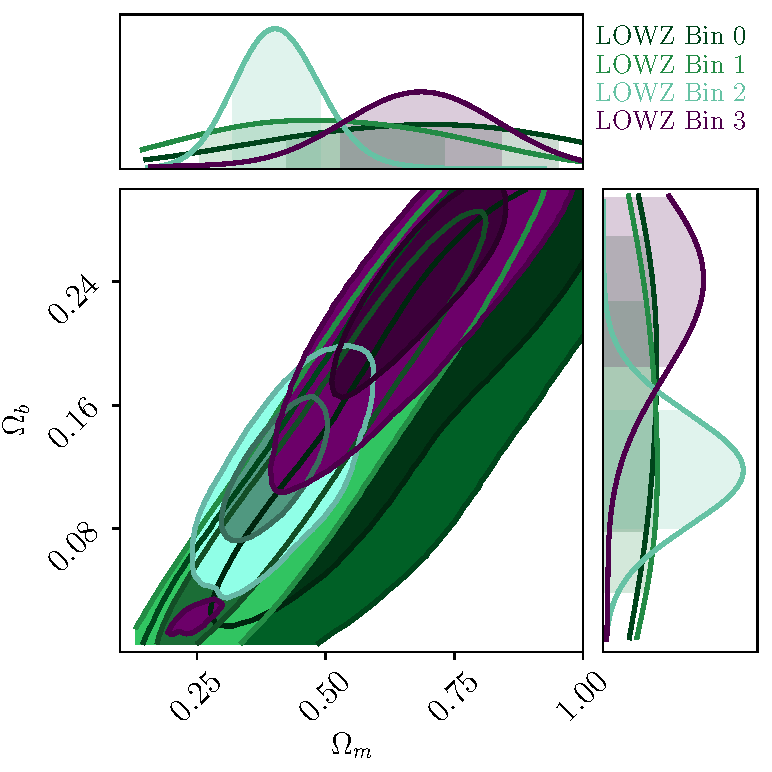
\includegraphics[width=\columnwidth]{BOSS-FIGS/LOWZ_SINGLE_BIN_1.pdf}
  \caption{}
\end{subfigure}%
\begin{subfigure}{.5\textwidth}
  \centering
  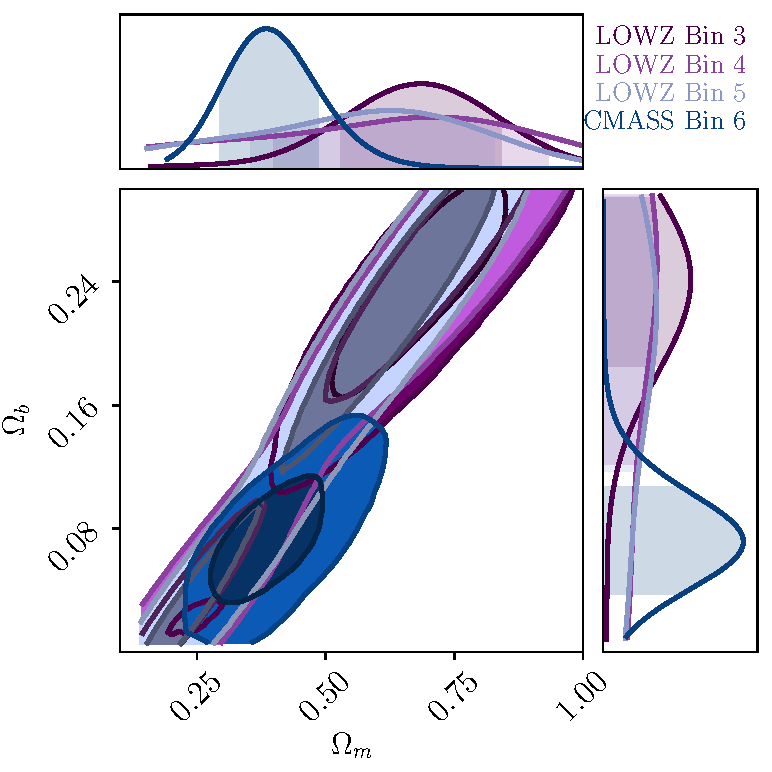
\includegraphics[width=\columnwidth]{BOSS-FIGS/LOWZ_SINGLE_BIN_2.pdf}
  \caption{}
\end{subfigure}\\
\begin{subfigure}{.5\textwidth}
  \centering
  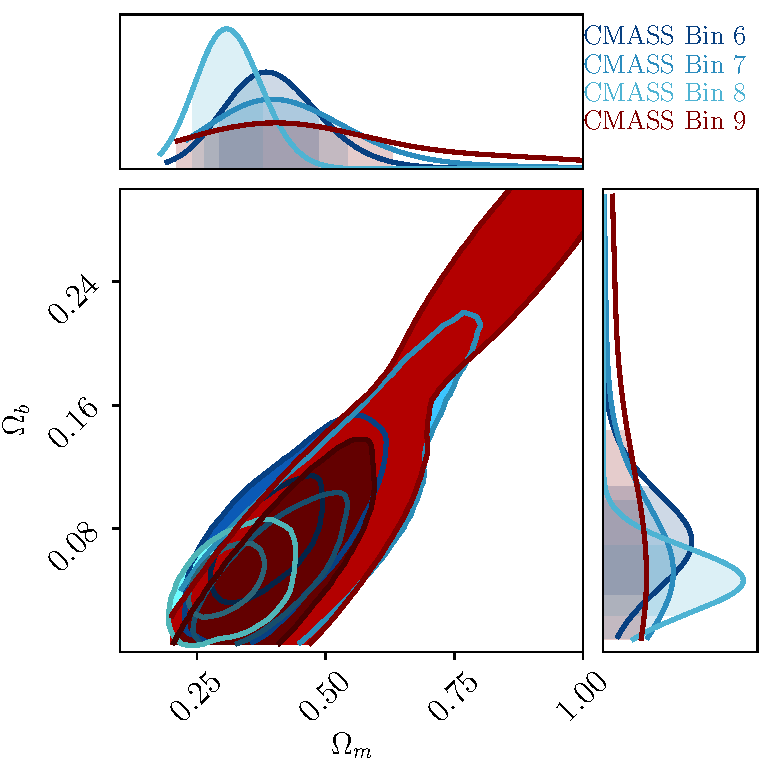
\includegraphics[width=\columnwidth]{BOSS-FIGS/CMASS_SINGLE_BIN_1.pdf}
  \caption{}
\end{subfigure}%
\begin{subfigure}{.5\textwidth}
  \centering
  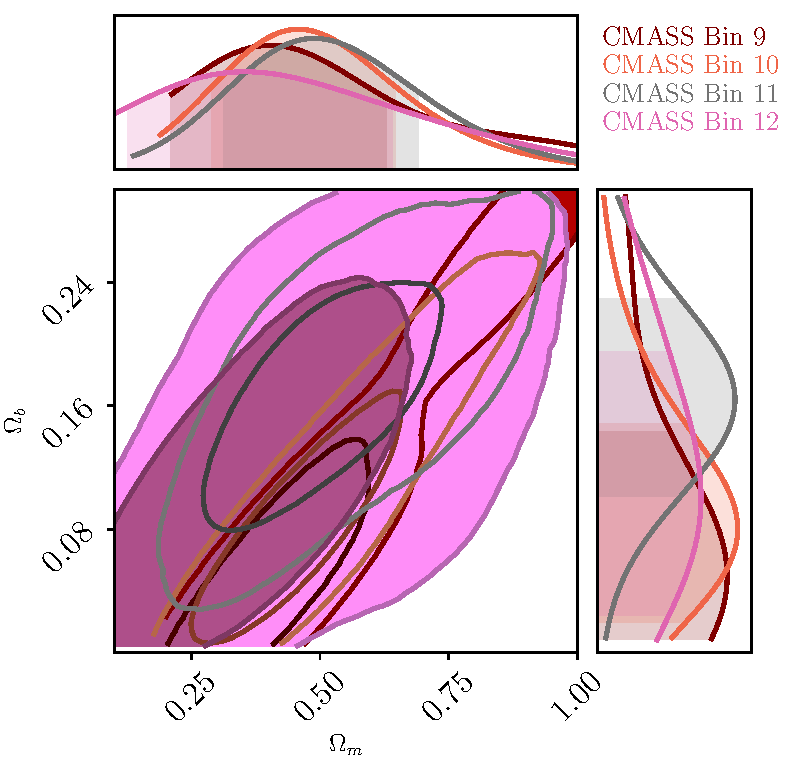
\includegraphics[width=\columnwidth]{BOSS-FIGS/CMASS_SINGLE_BIN_2.pdf}
  \caption{}
\end{subfigure}%
\caption[Consistency checks for single tomographic redshift bins for all LOWZ and CMASS bins using the $\Omega_b\,  \times \, \Omega_{m}$ contours]{Consistency checks for single tomographic redshift bins for all LOWZ and CMASS bins. Here, I show the $\Omega_b\,  \times \, \Omega_{m}$ contours taken from a $\Lambda$CDM cosmological inference, i. e. varying the same cosmological parameters as the ones from Section \ref{Sec:LCDM}. \textit{(a)} Shows LOWZ-0, LOWZ-1, LOWZ-2, and LOWZ-3 tomographic bins; \textit{(b)} shows LOWZ-3, LOWZ-4, LOWZ-5, and CMASS-6 tomographic bins; \textit{(c)} shows CMASS-6, CMASS-7, CMASS-8, and CMASS-9 tomographic bins; and \textit{(d)} shows CMASS-9, CMASS-10, CMASS-11, and CMASS-12 tomographic bins.}
\label{fig:SiingleBinAnaly}
\end{figure}

\subsection{Distribution of Residuals}
For a dataset with uncorrelated errors (diagonal covariance matrix), the vector of normalised residuals is given by:

\begin{equation}
R = \Xi^{-1}(D - T(\vec{\theta}))
\label{Eq:Residuals_1}
\end{equation}
where $\Xi$ is a diagonal matrix containing the square roots of the variances, $D$ is the data vector and $T(\vec{\theta})$ is the theory vector for a given parameter vector $\vec{\theta}$. If $T(\vec{\theta})$ represents the true model, and the true errors are known, the residuals are by definition given by a Gaussian with $\mu=0$ and $\sigma=1$ \citep{chisq2010}. On the other hand, if the errors are estimated from the data, the residuals are given by a Student's t-distribution. This distribution approaches a Gaussian with increasing number of data points. If this distribution shows a significant deviation from a Gaussian, the model is ruled out. If it follows a Gaussian distribution, one either found the true model, or the current data is not enough to distinguish between the model found and the true model \citep{chisq2010}.

\qquad When the covariance matrix is not diagonal (the errors are correlated), Equation \eqref{Eq:Residuals_1} is no longer true and one has to deal with the full covariance matrix. In order to get back to a diagonal matrix, the covariance matrix can be written in terms of its eigen-decomposition :

\begin{equation}
C = Q \Lambda Q^{-1}
\end{equation}
where $Q$ is the matrix of eigenvectors and $\Lambda$ is the diagonal matrix containing the eigenvalues of $C$. The inverse is then given by $C^{-1} = Q \Lambda^{-1} Q^{-1}$, which transforms the $\chi^2$ into:

\begin{equation}
\chi^2 = \big[ \hat{S}_{\Delta\ell} - S^{th}_{\Delta\ell}(\pmb{\Theta}, \pmb{\nu})\big]^T Q \Lambda^{-1} Q^{-1} \big[ \hat{S}_{\Delta\ell} - S^{th}_{\Delta\ell}(\pmb{\Theta}, \pmb{\nu})\big]
\end{equation}
If $\Lambda$ is treated as the new (diagonal) covariance matrix, it follows that the normalised residuals are now given by:

\begin{equation}
R = \Xi^{-1} Q^{-1} \big[ \hat{S}_{\Delta\ell} - S^{th}_{\Delta\ell}(\pmb{\Theta}, \pmb{\nu})\big]
\label{Eq:Residuals_2}
\end{equation}
where $\Xi$ now contains the square roots of the eigenvalues.%($\sqrt[]{\lambda_n}$). 

\qquad In this test, Equation \eqref{Eq:Residuals_2} is used to calculate the residuals at the best-fit point in a flat $\Lambda CDM$ Cosmology and plot the results in a histogram (Figure \ref{fig:Residuals}). There are no significant deviations from a Gaussian with $\mu=0$ and $\sigma=1$, which means the model seems to be a very good representation of the data.

\begin{figure}
\begin{center}
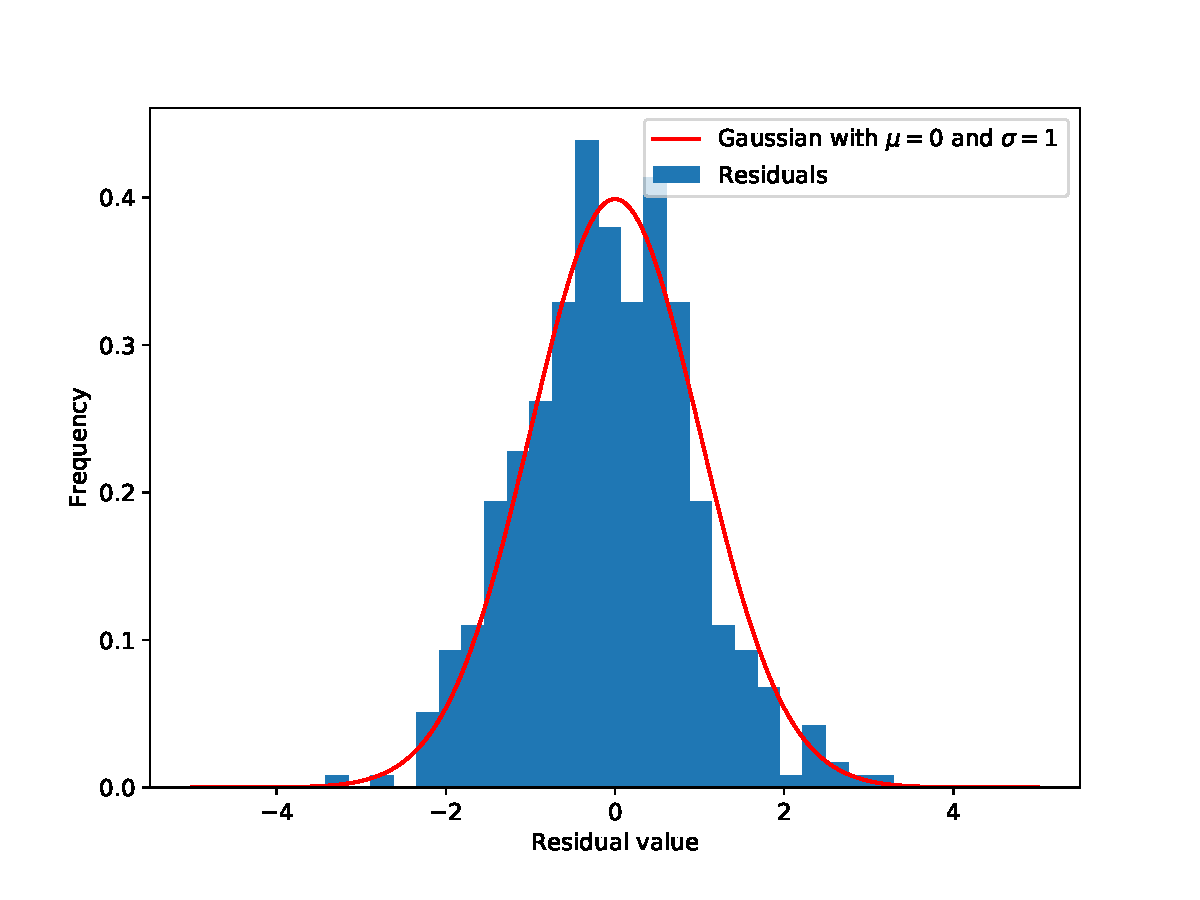
\includegraphics[scale=0.60]{BOSS-FIGS/chi_lcdm_new.pdf}
\caption[Distribution of residuals for the best-fit point in a flat $\Lambda$CDM models.]{Comparison between the histogram of the distribution of residuals (given by Equation \eqref{Eq:Residuals_2}) calculated at the best-fit point in a flat $\Lambda$CDM cosmology (see Section \ref{Sec:LCDM}) and a Gaussian with $\mu=0$ and $\sigma=1$. As this distribution does not show any significant deviation from the Gaussian, the model is either the truth or the current data cannot make any further distinction between the model and the truth.} 
\label{fig:Residuals}
\end{center}
\end{figure}

\section{External data}\label{Sec:ExternalData}

I compared and combined the results in this chapter with results obtained from the Planck satellite CMB experiment \citep{PlanckResults2015}, and Type Ia Supernovae from the Joint Light curve Analysis (JLA) collaboration \citep{JLAdata}. The relevant likelihood codes for these probes were implemented and tested in the \uclcl pipeline. The results from these external datasets were checked against the official cosmological results from the relevant collaborations. I have recovered the published cosmological parameters with the \uclcl pipeline which allowed me to use and combine them with the BOSS angular power spectra.

\qquad The CMB data from Planck was added through the Planck likelihood codes \texttt{Commander} and \texttt{Plik} \citep{PlanckLikelihood2015}. For low multipoles, in the range $l=2-29$, \texttt{Commander} is used with temperature (TT) and polarization auto- and cross- power spectra (BB, TB, EB). For high multipoles, in the range $l=30-2508$, \texttt{Plik} is used with temperature (TT) and polarization auto- and cross- power spectra (TE, EE). This configuration is commonly referred to as Planck TT,TE,EE+lowP. \texttt{Plik} also introduces 94 additional nuisance parameters. In order to reduce this large parameter space, the lite version of the data offered by the Planck Collaboration was used. This lite version allows to compute a nuisance marginalized CMB likelihood. The only CMB nuisance parameter left is the Planck absolute calibration parameter ($y_{cal}$). I sample this parameter in all the runs that include Planck data. The Planck likelihood codes were added to \texttt{UCLPI} and all the Planck results presented have been obtained using this pipeline. I show in the all cosmological contours and in table \ref{tab:LCDM_Constraints} that this pipeline reproduces the cosmological results found by the Planck Collaboration \citep{PlanckCosmology2016}.

\qquad The SN data from JLA was added to the \texttt{UCLPI} pipeline through the likelihood code provided by the JLA Collaboration \citep{JLAdata}. This likelihood code needs the luminosity distances to the 740 Supernovae in the sample and 4 nuisance parameters ($\alpha, \beta, M_B, \Delta_M$) described in \cite{JLAdata}. The luminosity distances are calculated by \class \citep{Class} using the redshifts of the supernovae within a given Cosmology (set by the sampled cosmological parameters). I sample the absolute magnitude at peak brightness ($M_B$) as part of the analysis, and keep the other 3 nuisance parameters fixed to their best-fit values found by \cite{JLAdata} since these have a small impact in the cosmological parameters when combined with the BOSS dataset.

\qquad I also implemented a BAO likelihood in order to compare my results with the official \textbf{BOSS Consensus} results from \cite{2016BOSSCosmology}. This measurements use 3 redshift bins with $z_{eff} = 0.38, \, 0.51, \, \text{and} \, 0.61 $, where I used the full shape post-reconstruction measurements from the correlation function and 3D power spectra, which contains additional information from measurements of $f\sigma_8$ (see table 7 from \cite{2016BOSSCosmology}). I have not combined these results with my BOSS results, but I plot them alongside my results alone in the next sessions to give the reader an impression of how my results compare with the BOSS alone results from \cite{2016BOSSCosmology}.

%-----------------------------------------------------------------------%
%                        	COSMOLOGY: LCDM
%-----------------------------------------------------------------------%
\section{Cosmological Analysis}\label{Sec:CosmoAnal}
\subsection{Flat $\Lambda$CDM Constraints}\label{Sec:LCDM}
Here, I obtain constraints for the standard cosmological model, a flat $\Lambda$CDM cosmology. I fixed the curvature of the universe to zero, e.g. $\Omega_k = 0$, and varied five cosmological parameters: the baryonic density, $\Omega_b$; the dark matter density, $\Omega_{cdm}$; the amplitude of the primordial power spectra, $A_s$; the spectral index, $n_s$; and the Hubble constant, $h$. As this model considers dark energy as the cosmological constant $\Lambda$, I fixed the $w_0$ parameter to a cosmological constant ($w_0 = -1$), therefore: $\Omega_{\Lambda} = 1 - (\Omega_b + \Omega_{cdm})$. Here, I also fixed the sum of neutrino masses to the minimum found from neutrino oscillation experiments, $\sum m_{\nu} = 0.06 \, eV$ -- the lower bound as suggested from neutrino oscillation experiments \citep{2006NeutrinoReview,2014NeutrinoCosmoPlanck}. Following, I also obtained derived parameters as the total matter density, $\Omega_m \equiv \Omega_b + \Omega_{cdm}$; and the fluctuation of amplitude at 8 $h^{-1}$Mpc, $\sigma_8$ or $S_8 = \sigma_8\sqrt{\Omega_m/0.3}$. Finally, as described in the previous section, I varied the BOSS, Planck and JLA nuisance parameters. For this analysis, I used the $\ell_{max}^{5\%}$ cuts (see table \ref{Tb:EllCuts}).

\qquad I checked the consistency of the datasets by running the same analysis for these probes alone and combined (Planck, JLA, and Planck plus JLA) and calculating the respective Bayes factors for these cosmological constraints. The Bayes factor, Equation \eqref{Eq:BayesFactor},  for combinations of the considered datasets indicates consistency between all three probes:

\begin{align}
R_{\scriptscriptstyle\text{BOSS+JLA}}^{\Lambda CDM} & \simeq 18  \\
R_{\scriptscriptstyle\text{BOSS+PLANCK}}^{\Lambda CDM} & \simeq 74 \\
R_{\scriptscriptstyle\text{PLANCK+JLA}}^{\Lambda CDM} & \simeq 11 \\
R_{\scriptscriptstyle\text{BOSS+PLANCK+JLA}}^{\Lambda CDM} & \simeq 4 \times 10^4
\end{align}
these indicate that the datasets are compatible for the considered model, given the chosen priors.

\begin{figure}
\begin{center}
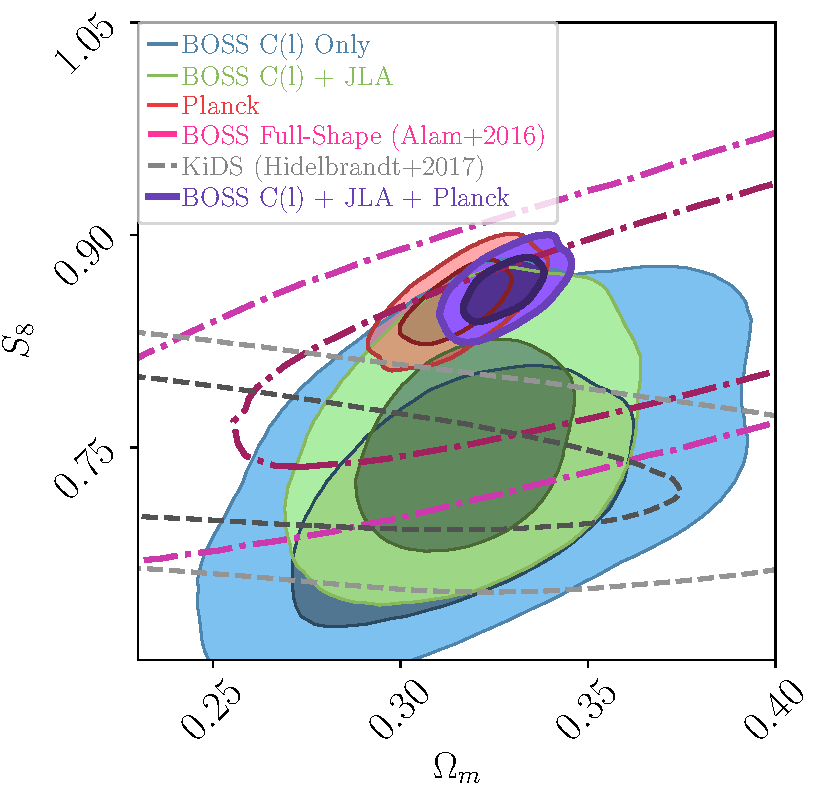
\includegraphics[scale=0.70]{BOSS-FIGS/LCDM_External_KidsOmega_m.pdf}
\caption[2D $\Omega_m \, \times \, S_8$ marginalised credible intervals for a $\Lambda$CDM cosmology.]{2D $\Omega_m \, \times \, S_8$ marginalised credible intervals for a \textbf{$\Lambda$CDM cosmology}. In this figure I show in detail the cosmological results from Section \ref{Sec:LCDM} for BOSS $C_{\ell}$s only \textit{(blue)}; BOSS $C_{\ell}$s plus JLA \textit{(green)}; BOSS $C_{\ell}$s plus JLA and Planck \textit{(purple)}; together with results using the post-reconstruction full shape (incl. $f\sigma_8(z)$) from \protect\cite{2016BOSSCosmology} consensus results \textit{(pink)}, and Planck alone \textit{(red)}. In order to compare these results to a weak-lensing probe, I also show here the results from \protect\cite{2017MNRAS.465.1454H} \textit{(grey, dashed)}. For details about the external datasets, see Section \ref{Sec:ExternalData}.}
\label{fig:Om_S8_LCDM}
\end{center}
\end{figure}

\qquad Finally, when considering the combination of BOSS $C_{\ell}$s, Planck and JLA, I find results consistent with \cite{2016BOSSCosmology,2017MNRAS.465.1454H,2017arXiv170801530D}. Figure \ref{fig:Om_S8_LCDM} shows the $\Omega_m \, \times \, S_8 $ 2D plane for this analysis and comparisons with Planck and the BOSS full-shape post-reconstruction from \cite{2016BOSSCosmology}. Despite the Bayes factors showing no significant reason to be concerned about the compatibility of these datasets, an interesting trend in this figure can be seen insofar as a tension and the BOSS dataset in this work preferring a smaller $S_8$ than the Planck analysis. I argue here that this method would prove potentially very useful in resolving any $S_8$ tensions which exist currently between CMB and weak lensing data \citep{2015MacCrann,2017CharnockTension}.

\qquad The results for the 1D marginalised cosmological constrains for BOSS $C_{\ell}$ and combinations, together with the 68\% credible intervals can be found in table \ref{tab:LCDM_Constraints}. The 1-$\sigma$ and 2-$\sigma$ contour levels can be found in Figure \ref{fig:LCDM_Cosmology} where the nuisance parameters have been marginalised over. Figure \ref{fig:Cl_Bestfit} shows the best fit theory $C_{\ell}$ using the parameters estimated from this analysis with a $\chi^2_{red} = 1.08$, which also indicates reliability and robustness of the analysis performed. 

\qquad Even though I do not show the results in this work, I performed a cosmological analysis using a $\Lambda$CDM with a fixed zero neutrino mass, $\sum m_{\nu} = 0$ eV. I compared it with the model used in this section, $\Lambda$CDM with $\sum m_{\nu}$ fixed to $0.06$ eV, using the Bayes factor for model selection. Consider $\vec{D}$ representing the combination of data vectors; the Bayes factor is given by

\EQ{}{
R_{A,B} = \frac{\mathcal{Z}(\vec{D}_{\scriptscriptstyle\text{BOSS+PLANCK+JLA}}|\sum m_{\nu} = 0.06 \text{ eV})}{\mathcal{Z}(\vec{D}_{\scriptscriptstyle\text{BOSS+PLANCK+JLA}}|\sum m_{\nu} = 0 \text{ eV}) } = 8\times 10^5
}
\noindent This indicates that, for a $\Lambda$CDM model, the data prefers massive neutrinos over no neutrino mass at all.


\begin{figure*}
\begin{center}
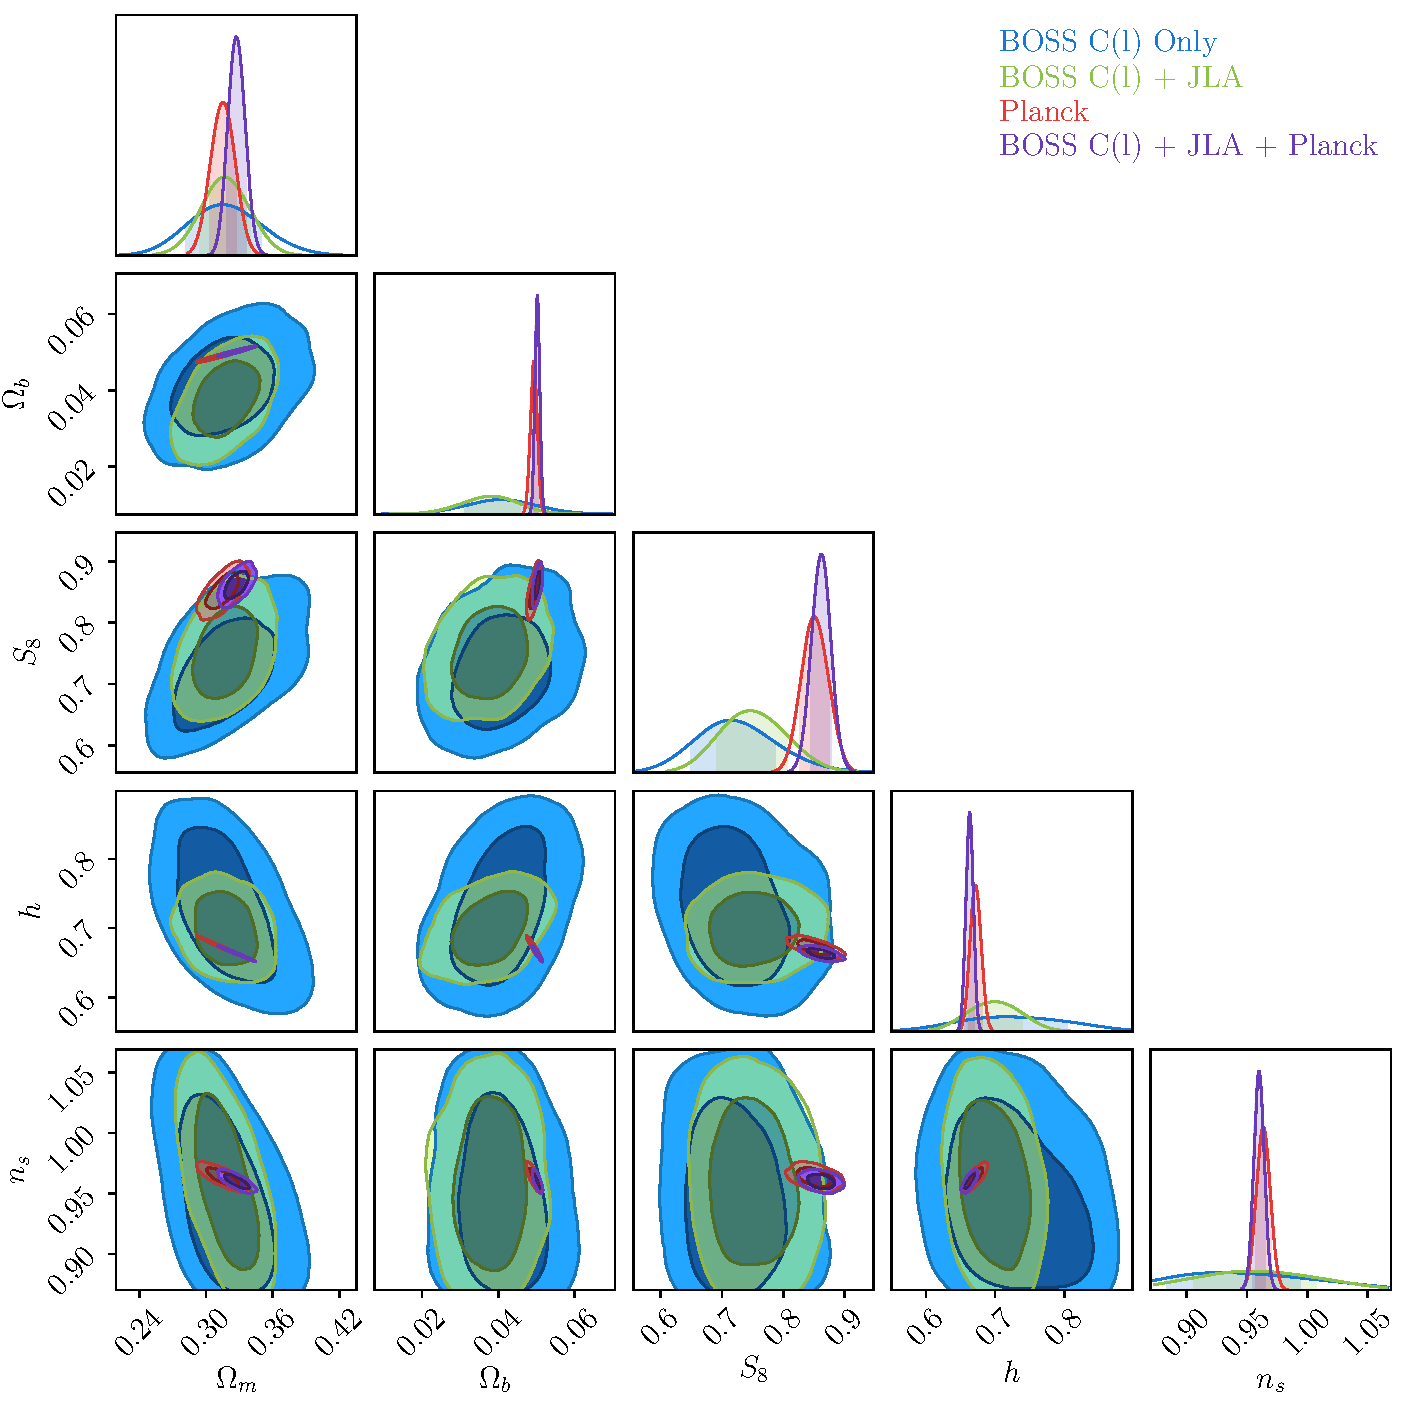
\includegraphics[width=\textwidth]{BOSS-FIGS/LCDM_Cosmology.pdf}
\caption[Marginalised 1 \& 2D cosmological constraints for the $\Lambda$CDM model.]{Marginalised 1 \& 2D cosmological constraints for the \textbf{$\Lambda$CDM model} varying five cosmological parameters with 1-$\sigma$ (darker) and 2-$\sigma$ (lighter) contour levels. I show here a combination of sampled and relevant derived parameters: $\Omega_m$, $\Omega_b$, $S_8$, $h$, and $n_s$ (marginalising over $\tau_{reio}$ for the Planck combinations). The \textit{blue contours} where estimated from the BOSS $C_{\ell}$s data alone using the SH16 likelihood; \textit{the green contours} are a combination the BOSS likelihood and JLA data (see Section \ref{Sec:ExternalData}); \textit{the red contours} are the Planck high-$\ell$ TT, TE, EE and low-$\ell$ P likelihood results (see Section \ref{Sec:ExternalData}); finally, the purple contours are a combination of the three probes: BOSS $C_{\ell}$, JLA and Planck (also high-$\ell$ TT, TE, EE and low-$\ell$ P). Note that none of the results here use Planck Lensing data.}
\label{fig:LCDM_Cosmology}
\end{center}
\end{figure*}

\begin{figure*}
\begin{center}
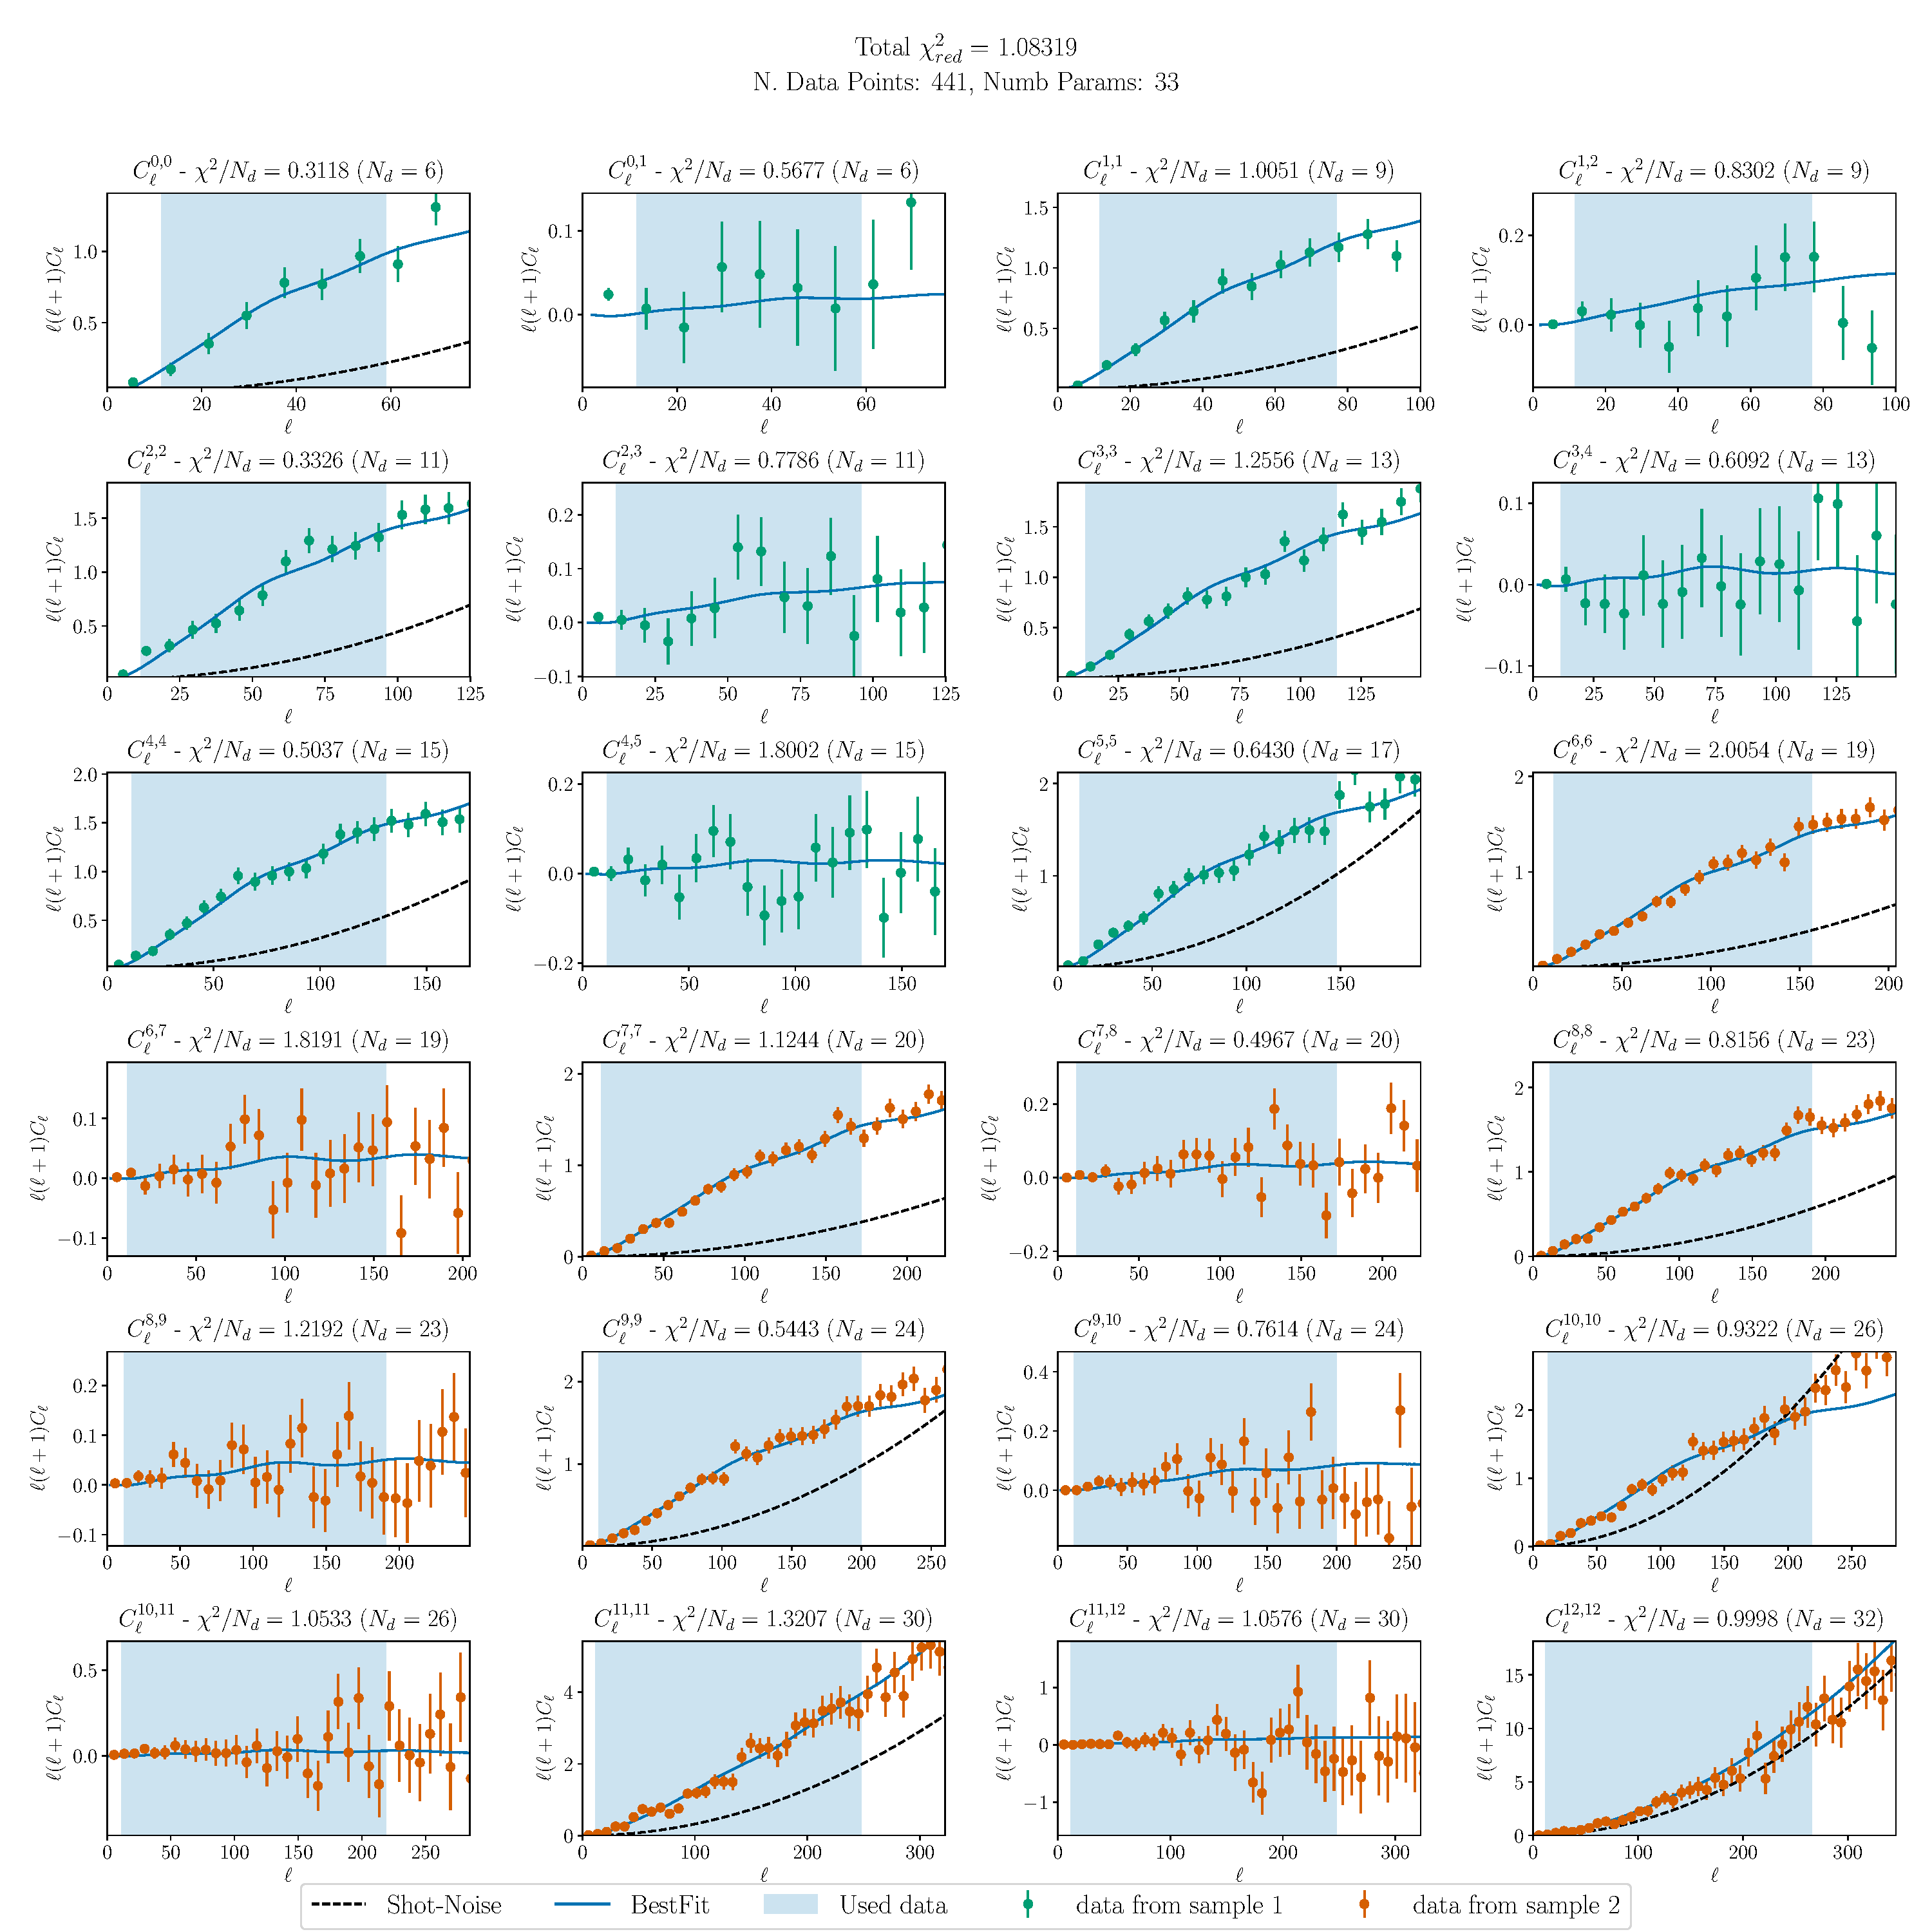
\includegraphics[width=1.05\columnwidth]{BOSS-FIGS/BestFit_LCDM.pdf}
\caption[BOSS measured $C_{\ell}$s and the best-fit theory from the $\Lambda$CDM model.]{Auto- and cross- angular power spectra for the 13 tomographic redshift bins considered for the BOSS DR12 samples: LOWZ (sample 1) and CMASS (sample 2). The shaded blue regions show the scales considered in the cosmological parameter estimation in Section \ref{Sec:CosmoBananas}. The \textit{data points} are the pseudo-$C_{\ell}$ estimates, described in Section \ref{Sec:Measurements}, for LOWZ and CMASS. The \textit{solid blue lines}, generated with \texttt{UCLCL}, reflect the \textit{best fit} auto- and cross-power spectra for the \textbf{$\Lambda$CDM model} estimated in Section \ref{Sec:LCDM}. Finally, the \textit{black dashed lines} show both shot noise and sampled shot noise (for bins 11 and 12). The overall reduced $\chi^2$ for this fit is $\chi^2_{red} \approx 1.08$, where the number of data points is 441 and the total number of sampled parameters is 33 -- 5 Cosmological parameters, and 28 nuisance parameters. The title on each individual plot reflects the bins \textit{i \& j} for each $C^{ij}_{\ell}$, the $\chi^2$ per data point ($\chi^2/N_d$), and the number of data points for that individual angular power spectrum, $N_d$. The $\ell$-ranges used in this figure correspond to the $\ell_{max}^{5\%}$ in table \ref{Tb:EllCuts}. Most of the constraining power comes from the auto-power spectra. The cross-power spectra serve to constrain parameters related to the RSD by helping to break the degeneracy between the bias and $A_s$ while also probing the redshift dispersion due to the peculiar motion of galaxies (FoG).}
\label{fig:Cl_Bestfit}
\end{center}
\end{figure*}


%------------------------------------------------------------------------%
%                        	COSMOLOGY: wCDM
%------------------------------------------------------------------------%

\subsection{Flat $w$CDM Constraints}\label{Sec:wCDM}
In this section, I allowed the equation-of-state of dark energy, $w_0$, to vary. This is a trivial extension of the standard model of cosmology with just one extra parameter. If $w_0 = -1$, the solution indicates that the nature of dark energy is actually the cosmological constant, $\Lambda$. The procedure for this analysis followed in similar fashion as the one outlined in Section \ref{Sec:LCDM}, varying six parameters instead of five: $\Omega_b$, $\Omega_{cdm}$, $n_s$, $\ln 10^{10} A_s$, $h$, and the extra $w_0$. Note that, for this case, I am not varying $w_a$, i. e., I do not consider a redshift evolution in the equation-of-state of dark energy. Again, I fixed the neutrino parameter to $\sum m_{\nu} = 0.06 \, eV$ \citep{2006NeutrinoReview,2014NeutrinoCosmoPlanck}. Here, I used the same $\ell_{max}^{5\%}$ cuts as in the last section (see table \ref{Tb:EllCuts}).

\begin{figure}
\begin{center}
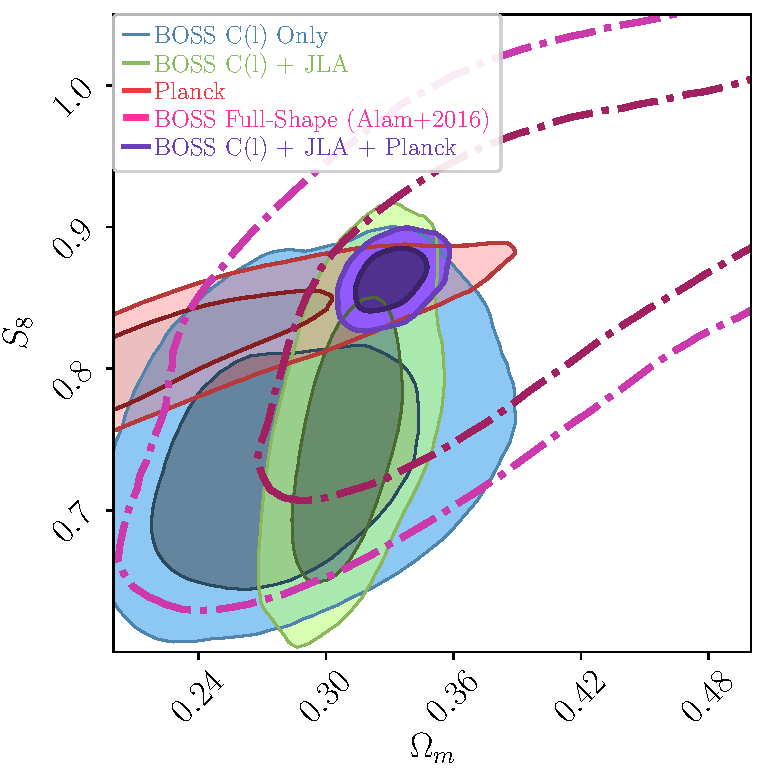
\includegraphics[scale=0.70]{BOSS-FIGS/Om_S8_wCDM.pdf}
\caption[2D $\Omega_m \, \times \, S_8$ marginalised credible intervals for a $w$CDM Cosmology.]{2D $\Omega_m \, \times \, S_8$ marginalised credible intervals for a \textbf{$w$CDM Cosmology}. This shows in detail the cosmological results from Section \ref{Sec:wCDM} for BOSS $C_{\ell}$s only \textit{(blue)}; BOSS $C_{\ell}$s plus JLA \textit{(green)}; BOSS $C_{\ell}$s plus JLA and Planck \textit{(purple)}; together with results using just the full shape (pre-reconstruction) from \protect\cite{2016BOSSCosmology} consensus results \textit{(pink)}, and Planck alone \textit{(red)}.}
\label{fig:Om_S8_wCDM}
\end{center}
\end{figure}

\qquad Figures \ref{fig:Om_S8_wCDM} and \ref{fig:Om_w0_wCDM} show in detail the contours for $S_8 \, \times \, \Omega_m$ and $w_0 \, \times \, \Omega_m$, respectively, and comparisons with previous measurements in the literature. From the Figure \ref{fig:Om_w0_wCDM} and from the complete set of results in \ref{fig:wCDM_Cosmology} I show that a $\sim 4\%$ error (1-$\sigma$ CI) on the equation-of-state of dark energy is obtained from this cosmological analysis:

\EQ{w0PlankBOSSJLA}{w_0 = -0.993^{+0.046}_{-0.043}.}
This results is consistent with the $\Lambda$CDM scenario of standard cosmology, i. e., it is consistent with dark energy being a cosmological constant, $\Lambda$. Note from Figure \ref{fig:wCDM_Cosmology} that I find a small value of $h$ (compared to \citealt{PlanckCosmology2016}) when combining BOSS $C_{\ell}$s, Planck, and JLA:

\EQ{}{h^{w\text{CDM}} = 0.661\pm 0.012.} This value is lower than the quoted Planck value alone; putting further tension in of this result if compared to the Hubble constant result from Cepheid Variables \citep{Riess2016, Riess2018}. 

\begin{figure}
\begin{center}
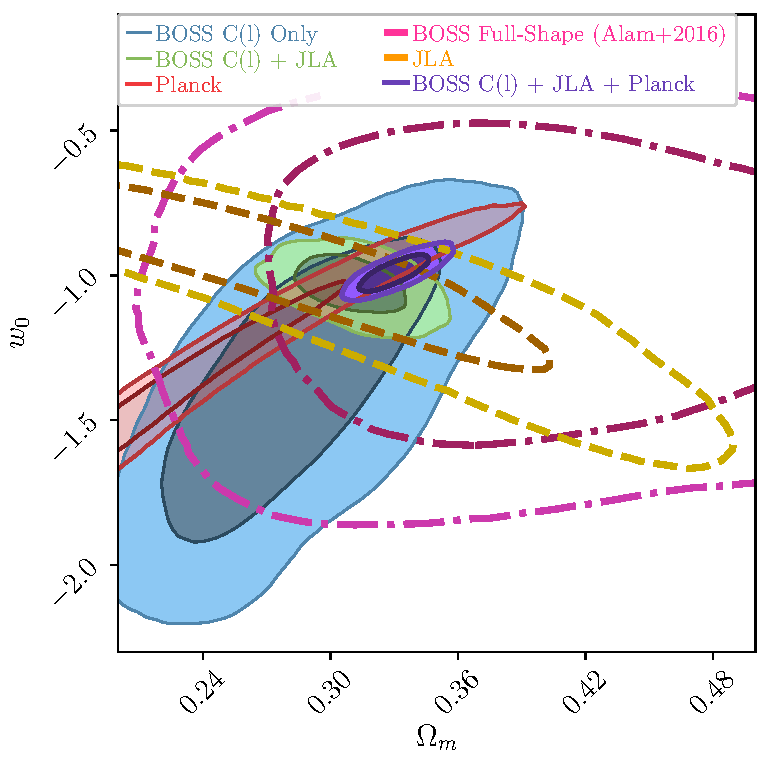
\includegraphics[scale=0.70]{BOSS-FIGS/w0_Om_wCDM.pdf}
\caption[2D $w_0 \, \times \, \Omega_m$ marginalised credible intervals for a $w$CDM Cosmology.]{2D $w_0 \, \times \, \Omega_m$ marginalised credible intervals for a \textbf{$w$CDM Cosmology}. This shows in detail the cosmological results from Section \ref{Sec:wCDM} for BOSS $C_{\ell}$s only \textit{(blue)}; BOSS $C_{\ell}$s plus JLA \textit{(green)}; BOSS $C_{\ell}$s plus JLA and Planck \textit{(purple)}; together with results using just the full shape (pre-reconstruction) from \protect\cite{2016BOSSCosmology} consensus results \textit{(pink)}, JLA \textit{(yellow)}, and Planck alone \textit{(red)}.}
\label{fig:Om_w0_wCDM}
\end{center}
\end{figure}

\qquad As the model in this section is different from the previous section, I performed an evidence analysis using the Bayes factor, Equation \eqref{Eq:BayesFactor}, in order to be sure that the measurements can be combined with the the external data described in Section \ref{Sec:ExternalData}. The following Bayes factors indicate that such combinations are consistent:

\begin{align}
R_{\scriptscriptstyle\text{BOSS+JLA}}^{\textit{w}CDM} & \simeq 2 \times 10^2  \\
R_{\scriptscriptstyle\text{BOSS+PLANCK}}^{\textit{w}CDM} & \simeq 4 \times 10^3 \\
R_{\scriptscriptstyle\text{PLANCK+JLA}}^{\textit{w}CDM} & \simeq 2 \\
R_{\scriptscriptstyle\text{BOSS+PLANCK+JLA}}^{\textit{w}CDM} & \simeq 3 \times 10^5
\end{align}

Finally, I used the ratio of the evidences, the Bayes factor, to perform a model selection between $w$CDM and $\Lambda$CDM using the final dataset combination. Assuming $\vec{D}$ to be the combination of data vectors for all the datasets, the Bayes factor between the two models is
\EQ{}{
R_{w,\Lambda} = \frac{\mathcal{Z}(\vec{D}_{\text{BOSS+Planck+JLA}}|w\text{CDM})}{\mathcal{Z}(\vec{D}_{\text{BOSS+Planck+JLA}}|\Lambda\text{CDM})} = 0.67
}
which does not significantly mean that one of the models is preferred over the other.

\begin{figure*}
\begin{center}
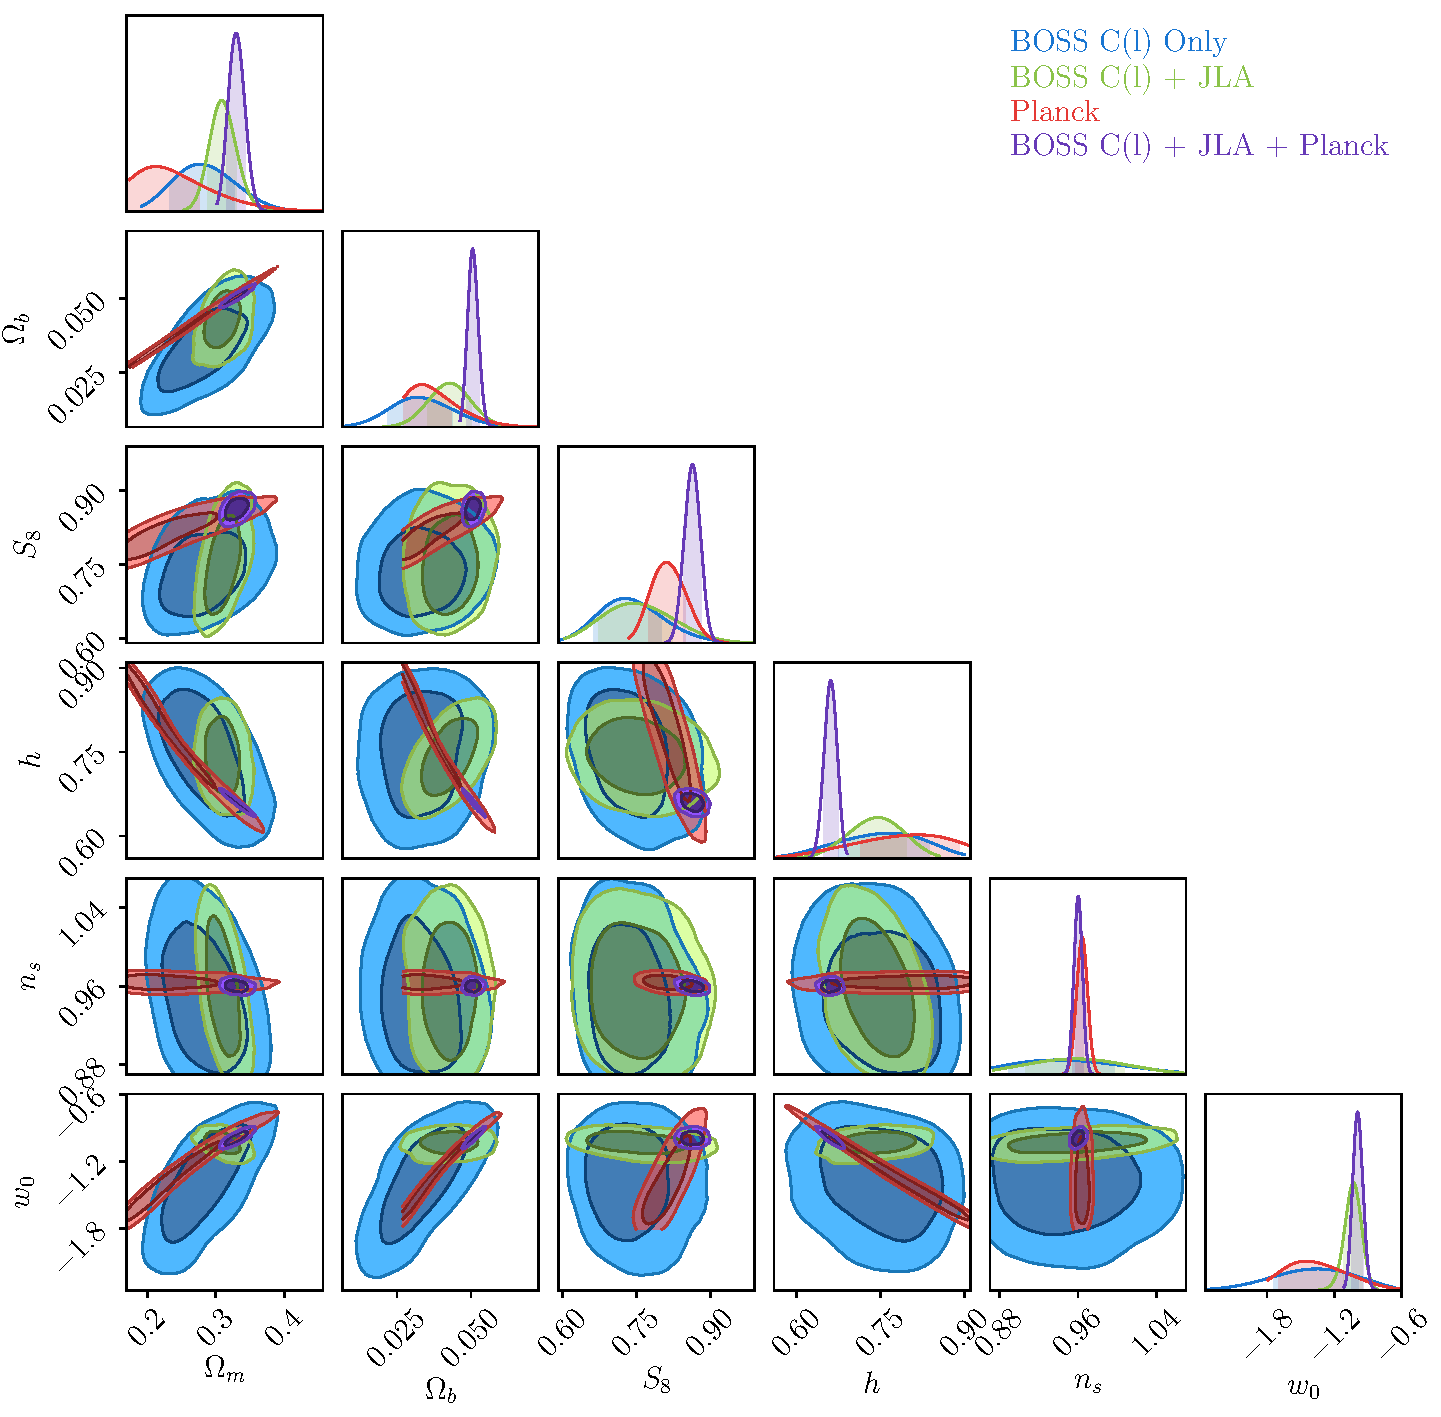
\includegraphics[width=\textwidth]{BOSS-FIGS/wCDM_Cosmology.pdf}
\caption[Cosmological constraints for the $w$CDM model.]{Cosmological constraints for the \textbf{$w$CDM model} varying now six cosmological parameters. This figure contains a combination of sampled and relevant derived parameters from the chains: $\Omega_m$, $\Omega_b$, $S_8$, $h$, $n_s$, and $w_0$. Note that the Planck chains also varied $\tau_{reio}$. The \textit{blue contours} where estimated from the BOSS $C_{\ell}$s data alone using the SH16 likelihood; \textit{green contours} are a combination the BOSS likelihood and JLA data; \textit{ red contours} are the Planck high-$\ell$ TT, TE, EE and low-$\ell$ P likelihood results; finally, the \textit{purple contours} are a combination of the three probes: BOSS $C_{\ell}$, JLA and Planck (also high-$\ell$ TT, TE, EE and low-$\ell$ P). The apparent cuts in the Planck alone contours are due to the prior in $h$. Note, again, that none of the results here use Planck Lensing data.}
\label{fig:wCDM_Cosmology}
\end{center}
\end{figure*}

%------------------------------------------------------------------------%
%                        	COSMOLOGY: LCDM + NEUTRINOS
%------------------------------------------------------------------------%

\subsection{Flat $\Lambda$CDM + $\sum m_\nu$ Constraints}\label{Sec:nCDM}
For the last model considered in this work, I now assume a flat $\Lambda$CDM with variable neutrino masses, varying the sum of the species' masses, $\sum m_{\nu}$. In the previous sections, I have fixed the sum of neutrino masses to $\sum m_{\nu} = 0.06 \, eV$ due to results from neutrino oscillation experiments for the lower bound of the normal neutrino mass ordering \citep{2003HannestadNeutrino,2006NeutrinoReview,2016Hannestad}. Here, I considered one of the two different scenarios regarding different neutrino hierarchies, the \textit{normal hierarchy}.  To approximate the normal hierarchy, one can approximate the two lower masses to be zero and vary $\sum m_{\nu}$ for one remaining massive species. I do not investigate details of how the prior on the hierarchy or on the absolute mass change this result in this chapter  -- Chapter \ref{Chap:Neutrinos} will explore in more details the impact of model selection in the mass and hierarchy of neutrinos. I fix $N_{eff} = 3.046$ by changing the values of massive neutrinos and ultra-relativist particles for the case considered, i. e. $N_{\nu} = 1$ and $N_{ur} = 2.0328$.

\begin{figure}
\begin{center}
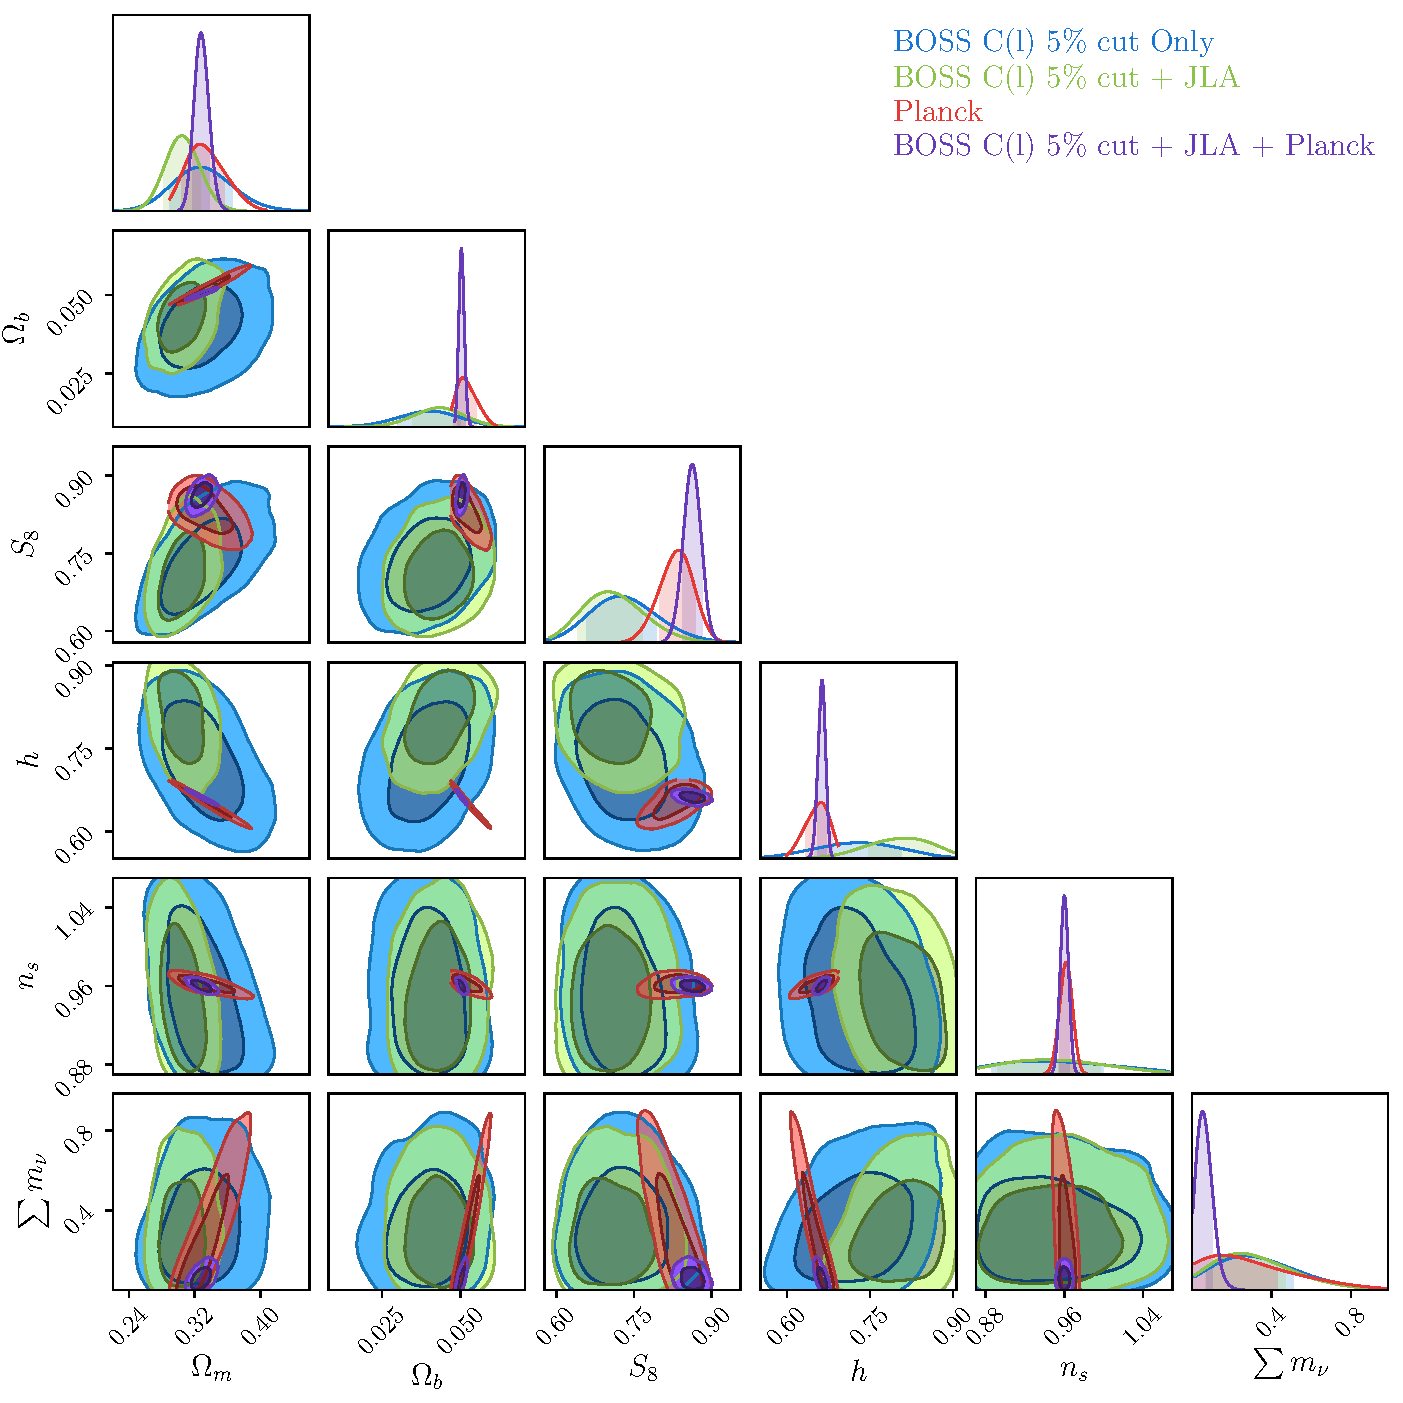
\includegraphics[width=\textwidth]{BOSS-FIGS/1Spec_Neutrino_NewPrior_LCDM_5pc.pdf}
\caption[1D and 2D marginalised credible intervals for a $\Lambda$CDM Cosmology with $\sum m_{\nu}$ when using scales up to $k_{max}\approx 0.07 h$ Mpc$^{-1}$]{1D and 2D marginalised credible intervals for a \textbf{$\Lambda$CDM Cosmology with $\sum m_{\nu}$} when using scales up to $k_{max}\approx 0.07 h$ Mpc$^{-1}$ ($\ell_{max}^{5\%}$ cut). Here I show the $\Omega_m$, $\Omega_b$, $S_8$, $h$, $n_s$, and $\sum m_{\nu}$ contours for BOSS $C_{\ell}$s alone \textit{(blue)}; BOSS $C_{\ell}$s plus JLA \textit{(green)}; Planck high-$\ell$ TT, TE, EE and low-$\ell$ P \textit{(red)}; and BOSS $C_{\ell}$s plus JLA and Planck high-$\ell$ TT, TE, EE and low-$\ell$ P \textit{(purple)}. As most of the scales that contain clean information on the neutrino masses are cut off, the 95\% CI upper bound found is $\sum m_{\nu} < 0.14$ eV.}
\label{fig:nuCDM5pc}
\end{center}
\end{figure}

\qquad Firstly, I perform an analysis using the same $\ell$-range as in the previous sections, $\ell_{max}^{5\%}$ from table \ref{Tb:EllCuts}. A summary for the marginalised 1D credible intervals from the cosmological estimation made with this cut can be found in the third part of table \ref{tab:LCDM_Constraints} showing the one sigma intervals for the $\Lambda$CDM parameters plus the 95\% upper limit for $\sum m_{\nu}$. The 1D and 2D marginalised credible intervals for this analysis can be found in Figure \ref{fig:nuCDM5pc}. When considering an approximation for the normal hierarchy, for a combination of BOSS $C_{\ell}$s, Planck CMB data, and supernovae data from JLA, the 95\% upper limit for sum of neutrino masses is:
\EQ{}{\sum m_{\nu} < 0.14 \, eV \quad \small\text{(BOSS + Planck + JLA -- $\ell_{max}^{5\%}$ cut)}}

\qquad From Figure \ref{fig:neutrinoCompare1} and even more so from Figure \ref{fig:neutrinoCompare2}, one can notice that this analysis is not so far from excluding zero total neutrino mass using cosmological data alone. As the power of such datasets increase it should be able, using the correct analysis and tools, to measure and detect neutrino masses independently from atmospheric experiments.

\qquad One more, I proceed to perform a consistency of datasets by using the evidence of each cosmological parameter estimation for these model to calculate the Bayes factor (Equation \ref{Eq:BayesFactor}). The following values, again, indicate the consistency of datasets for the considered model.
\begin{figure}
\begin{center}
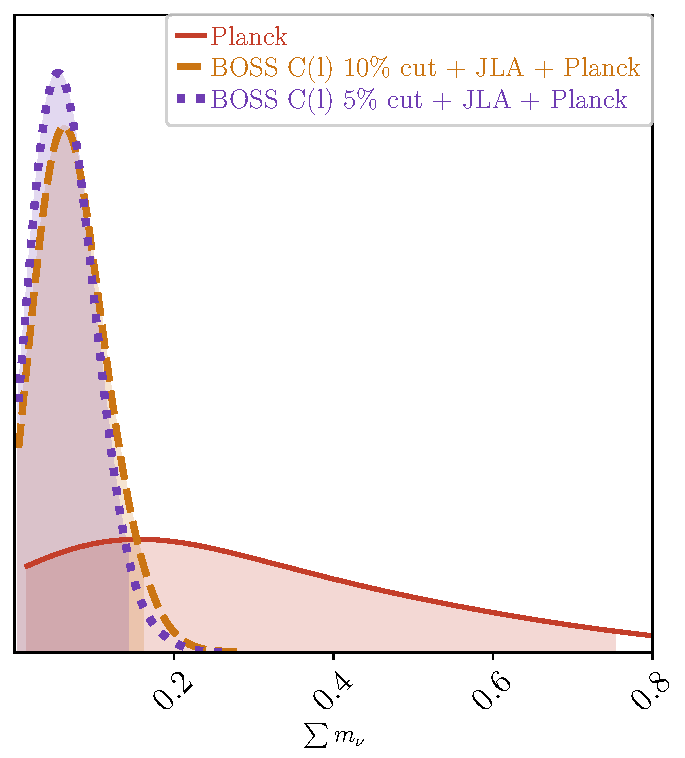
\includegraphics[scale=0.70]{BOSS-FIGS/neutrino_1D.pdf}
\caption[1D marginalised distribution with 95\% credible intervals for $\sum m_{\nu}$.]{1D marginalised distribution with 95\% credible intervals for $\sum m_{\nu}$ in three different cases: \textit{(red solid)} Planck high-$\ell$ TT, TE, EE and low-$\ell$ P, \textit{(yellow dashed)} BOSS $C_{\ell}$s with the $\ell_{max}^{10\%}$ cut plus Planck and JLA, and \textit{(purple dotted)} BOSS $C_{\ell}$s with the $\ell_{max}^{5\%}$ cut plus Planck and JLA. The 95\% upper limit for each case is, respectively: \textit{(red)} 0.76 eV, \textit{(yellow)} 0.16 eV, and \textit{(purple)} 0.14 eV.}
\label{fig:neutrinoCompare1}
\end{center}
\end{figure}
\begin{figure}
\begin{center}
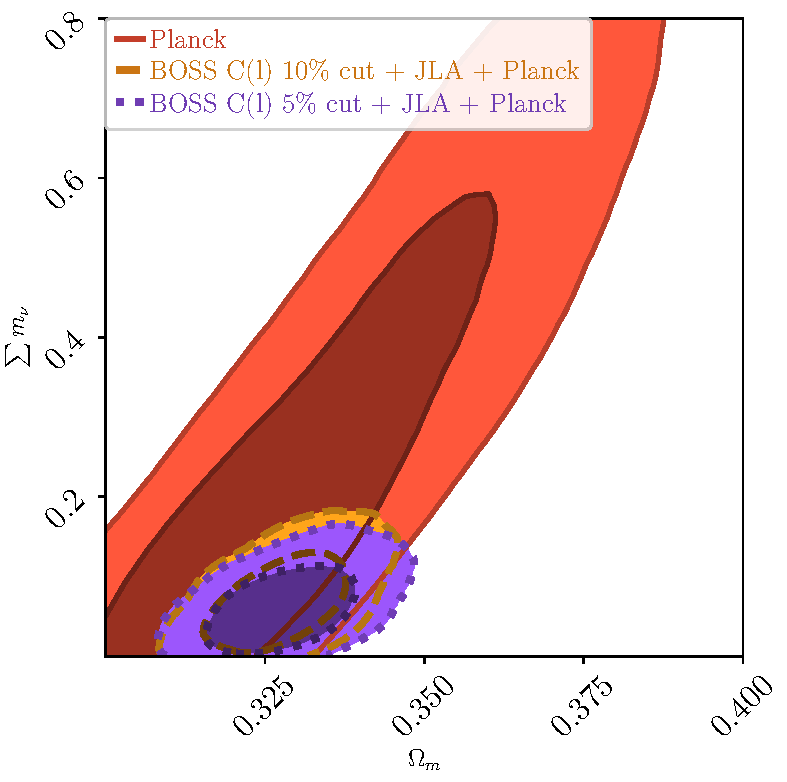
\includegraphics[scale=0.70]{BOSS-FIGS/neutrino_2D.pdf}
\caption[2D marginalised 1- and 2-$\sigma$ credible intervals for the $\sum m_{\nu}$-$\Omega_m$ plane.]{2D marginalised 1- and 2-$\sigma$ credible intervals for the $\sum m_{\nu}$-$\Omega_m$ plane for three different cases: \textit{(blue solid)} Planck high-$\ell$ TT, TE, EE and low-$\ell$ P, \textit{(red dashed)} BOSS $C_{\ell}$s with the $\ell_{max}^{10\%}$ cut plus Planck and JLA, and \textit{(orange dotted)} BOSS $C_{\ell}$s with the $\ell_{max}^{5\%}$ cut plus Planck and JLA.}
\label{fig:neutrinoCompare2}
\end{center}
\end{figure}

\begin{align}
R_{\scriptscriptstyle\text{BOSS+JLA}}^{\Lambda CDM + \sum m_{\nu} \, 5\%} & \simeq 1\times 10^2  \\
R_{\scriptscriptstyle\text{BOSS+PLANCK}}^{\Lambda CDM +\sum m_{\nu} \, 5\%} & \simeq 4\times 10^2 \\
R_{\scriptscriptstyle\text{PLANCK+JLA}}^{\Lambda CDM +\sum m_{\nu}} & \simeq 40 \\
R_{\scriptscriptstyle\text{BOSS+PLANCK+JLA}}^{\Lambda CDM +\sum m_{\nu} \, 5\%} & \simeq 3 \times 10^2
\end{align}
 

\qquad For the final analysis in this work, In want to investigate the impact of the chosen scale cuts in the neutrino mass upper bounds. To do it so, I extended the scales considered for the $\ell_{max}^{10\%}$ cuts (see table \ref{Tb:EllCuts} for details). This allows to access smaller scales that are still in the beginning of the so-called the weak non-linear regime \citep{Thomas2010Neutr,Bird2012}. Note that these scales are still larger than the scales that most collaborations use for power spectra or correlation function cosmological analysis \citep{Ho2012,2016BOSSCosmology,2017MNRAS.465.1454H,2017arXiv170801530D} -- \cite{2017arXiv170801530D}, for example, uses scales up to $0.78h$ Mpc $^{-1}$. In other words, one can be confident that the $\ell_{max}^{10\%}$ cuts are safe to be used, not using scales outside the weak non-linear regime. 


\qquad Using these second scale cuts, I then proceed to perform a similar cosmological analysis for a $\Lambda$CDM model with one massive species of neutrino, the approximation to the normal hierarchy. The 1D and 2D marginalised credible intervals for these final analysis can be find in Figure \ref{fig:nuCDM10pc} and the marginalised 68\% credible intervals for the $\Lambda$CDM parameters and the 95\% credible interval upper limit for $\sum m_{\nu}$ using this cut can be found in table \ref{tab:LCDM_Constraints}. The Bayes factors for this choice are shown below -- note that I have 2 further nuisance parameters in the $\ell_{max}^{10\%}$ cut as I checked that failure to add these reduces the Bayes factor significantly.
\begin{align}
R_{\scriptscriptstyle\text{BOSS+JLA}}^{\Lambda CDM + \sum m_{\nu} \, 10\%} & \simeq 70  \\
R_{\scriptscriptstyle\text{BOSS+PLANCK}}^{\Lambda CDM +\sum m_{\nu} \, 10\%} & \simeq 6 \times 10^2 \\
R_{\scriptscriptstyle\text{BOSS+PLANCK+JLA}}^{\Lambda CDM +\sum m_{\nu} \, 10\%} & \simeq 3 \times 10^5
\end{align}

\qquad This extended scale analysis demonstrates the robustness of the results presented in this section as the 95\% CI upper bound for $\sum m_{\nu}$ remains robust to these cuts (see Figures \ref{fig:neutrinoCompare1} and \ref{fig:neutrinoCompare2}):
\EQ{}{\sum m_{\nu} < 0.16 \, eV \quad \small\text{(BOSS + Planck + JLA -- $\ell_{max}^{10\%}$ cut)}.}



\begin{figure}
\begin{center}
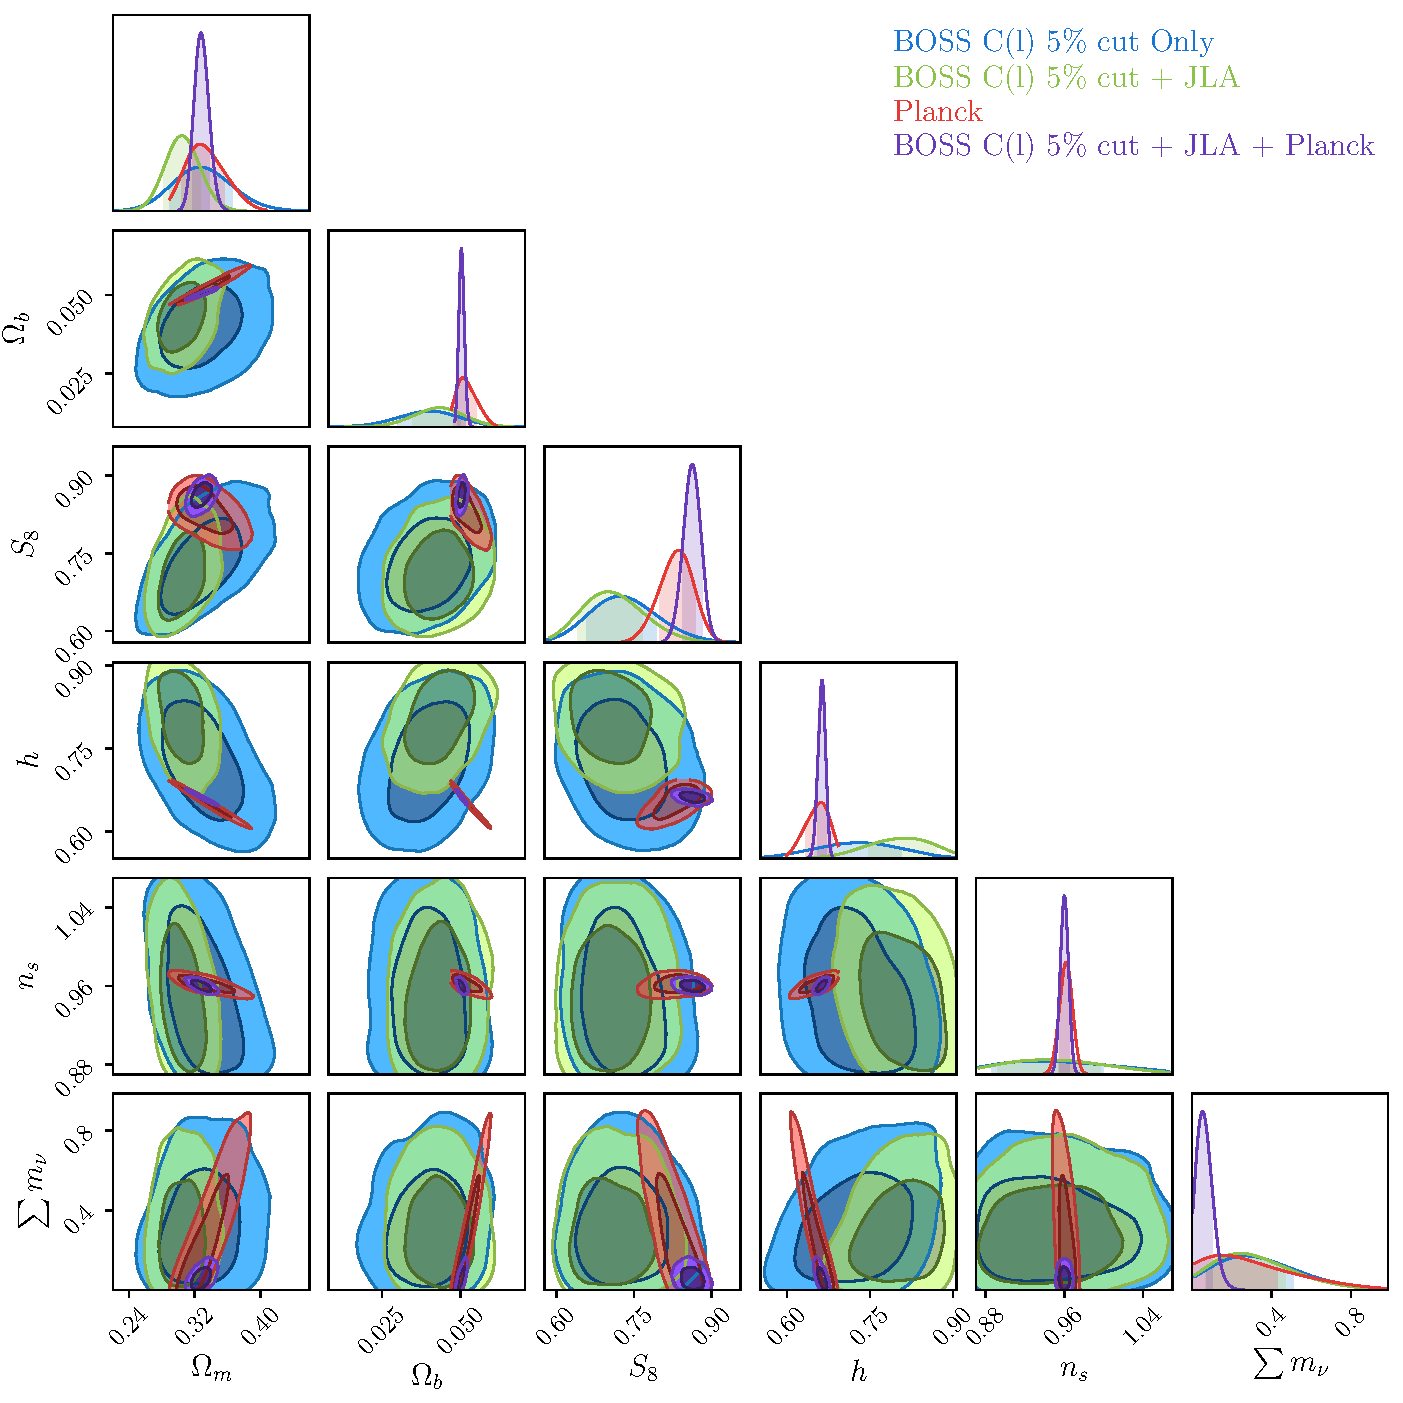
\includegraphics[width=\textwidth]{BOSS-FIGS/1Spec_Neutrino_NewPrior_LCDM_5pc.pdf}
\caption[Cosmological constraints for the $\Lambda$CDM + $\sum m_{\nu}$ model, using the $\ell_{max}^{10\%}$ cut]{Cosmological constraints for the \textbf{$\Lambda$CDM + $\sum m_{\nu}$ model}, using the $\ell_{max}^{10\%}$ cut, varying now six cosmological parameters, including the sum of neutrino masses considering only one massive species. This figure contains a combination of sampled and relevant derived parameters from the chains: $\Omega_m$, $\Omega_b$, $S_8$, $h$, $n_s$, and $\sum m_{\nu}$. Note that the Planck chains also varied $\tau_{reio}$. The \textit{blue contours} where estimated from the BOSS $C_{\ell}$s data alone using the SH16 likelihood; \textit{the green contours} are a combination the BOSS likelihood and JLA data; \textit{the red contours} are the Planck high-$\ell$ TT, TE, EE and low-$\ell$ P likelihood results; finally, the purple contours are a combination of the three probes: BOSS $C_{\ell}$, JLA and Planck (also high-$\ell$ TT, TE, EE and low-$\ell$ P). For this scale cut, the combination of datasets yields an upper bound on $\sum m_{\nu} < 0.16$eV.}
\label{fig:nuCDM10pc}
\end{center}
\end{figure}


\qquad A summary of all cosmological parameters estimated for all models and combinations of datasets can be found in table \ref{tab:LCDM_Constraints}.

%------------------------------------------------------------------------%
%                        CONCLUSIONS
%------------------------------------------------------------------------%
\section{Conclusions}
In this chapter, I produced several consistency checks which demonstrated the robustness of: the estimated covariance matrix, since the recovered cosmology was the same under different estimation methods (through simulation and theory); the likelihood, given it returns the same contours under three different approaches; and of the whole method, since I recovered the right cosmology using a controlled simulation.

\qquad Cosmological parameters were obtained for 3 different models: $\Lambda$CDM, $w$CDM, and $\Lambda$CDM with $\sum m_{\nu}$. I highlight the following main points regarding the results obtained in Section \ref{Sec:CosmoAnal}:
\begin{itemize}
\item[\textbf{1.}] The constraints obtained for all three models considered, using a tomographic analysis in harmonic space, are extremely competitive in comparison to the ones obtained by the BOSS Collaboration \citep{2016BOSSCosmology} and other recent big collaboration results such as DES \citep{2017arXiv170801530D} and KiDS \citep{2017MNRAS.465.1454H} with errors as small as the before-mentioned collaborations.

\item[\textbf{2.}] Even though information along the line-of-sight is ``washed away" due to projecting the data into tomographic bins, I obtain one of the tightest constraints for the  equation-of-state of dark energy with a $\sim$4\% error when combining BOSS $C_{\ell}$s, Planck CMB, and JLA Supernovae. This was never achieved before using $C_{\ell}$ with a spectroscopic survey and has constraints as tight as the one obtained from the state-of-the-art Dark Energy Collaboration analysis, using a combination of DES galaxy clustering \& weak lensing, Planck, JLA, and BAO \citep{2017arXiv170801530D}.

\item[\textbf{3.}] For the models and datasets considered, I find very high values for the Bayes factor, $R$, when combining BOSS $C_{\ell}$s, Planck, and JLA. I would like to highlight: $R_{\scriptscriptstyle\text{BOSS+PLANCK+JLA}} \simeq 4 \times 10^4$ for $\Lambda$CDM and $R_{\scriptscriptstyle\text{BOSS-10\%+PLANCK+JLA}} \simeq 3 \times 10^5$ for $\Lambda$CDM varying neutrino masses. 

\item[\textbf{4.}] The Bayes factor can also be used for model selection. Considering the combination of datasets, the Bayes factor between $\Lambda$CDM and $w$CDM is
\EQ{}{R_{w,\Lambda} = \frac{\mathcal{Z}(\vec{D}_{\text{BOSS+Planck+JLA}}|w\text{CDM})}{\mathcal{Z}(\vec{D}_{\text{BOSS+Planck+JLA}}|\Lambda\text{CDM})} = 0.67}
where $\vec{D}$ here just represents the overall combination of data vectors. This indicates that this combination prefers slightly more $\Lambda$CDM than $w$CDM, although no strong conclusion can be made. 

\item[\textbf{5.}] I find a small tension between BOSS $C_{\ell}$s and Planck for $S_8$ in all models considered with BOSS preferring smaller values. For example, for $\Lambda$CDM: 
\begin{align*}
S_8 & = 0.715^{+0.072}_{-0.064} \quad(\text{BOSS}) \\ \nonumber
S_8 &  = 0.850^{+0.023}_{-0.021}\quad(\text{Planck}) \nonumber
\end{align*}
although the combination of these datasets prefers higher values such as Planck (see table \ref{tab:LCDM_Constraints}) and the Bayes factor suggest the datasets are compatible. I conclude here that such tension can be investigated further with this method as LSS data increases in size and depth.

\item[\textbf{6.}] Although I do not show the contours in this chapter, I performed a cosmological analysis using a $\Lambda$CDM model but fixing $\sum m_{\nu} = 0 eV$ and compared with the $\Lambda$CDM results from Section \ref{Sec:LCDM}, which has a $\sum m_{\nu}$ fixed to $0.06$ eV. Using the Bayes factor for model selection, it is clear that the data prefers massive neutrinos against no neutrino mass at all:
\begin{align}
R_{0.06 eV, 0} & = \frac{\mathcal{Z}(\vec{D}_{\tiny\text{BOSS+Planck+JLA}}| \Lambda\text{CDM} + \sum m_{\nu} = 0.06)}{\mathcal{Z}(\vec{D}_{\tiny\text{BOSS+Planck+JLA}}| \Lambda\text{CDM} + \sum m_{\nu} = 0)} \nonumber \\
& = 8 \times 10^5 \nonumber
\end{align}

\item[\textbf{7.}] The neutrino mass constraints I obtain in this chapter can be compared to the tomographic analysis in real space done by \cite{2017SalazarBOSSwTheta}, which obtains an upper bound of $\sum m_{\nu} < 0.474$ eV (95\% CI). The reason I obtain much tighter constraints ($\sum m_{\nu} < 0.14$ eV (95\% CI)), even though I am also performing a tomographic analysis, is due to a series of decisions, including the approach I take to model the redshift dispersion and galaxy ``shell-crossing" (see Section \ref{Sec:SpecNz}), bias, and extra-shot noise. It is possible that the main difference between the results is due to different approach in modelling the neutrino mass hierarchy. In \cite{2017SalazarBOSSwTheta}, it is considered a model where the three neutrino species have degenerate mass hierarchy, i. e., the three masses are equal. This is already ruled out by particle physics experiments that measure the mass splitting from neutrino oscillation experiments (see \citealt{2014Gonzalez-GarciaNeutrino} for an update on the neutrino mass splitting fits). The approach I took in this chapter (see Section \ref{Sec:nCDM}) naturally yields smaller upper bounds in $\sum m_{\nu}$. In chapter \ref{Chap:Neutrinos}, I present a study about the impact of the model in the sum of neutrino masses and their hierarchy.

\end{itemize}


\begin{table}
    \centering 
    \caption[Marginalised cosmological constraints and 68\% credible intervals for the models considered in the BOSS analysis using a variety of datasets and combinations. ]{Marginalised cosmological constraints and 68\% credible intervals for the models considered in this work using a variety of datasets and combinations. The contours for these results are shown in Figures \ref{fig:LCDM_Cosmology} for $\Lambda$CDM, \ref{fig:wCDM_Cosmology} for $w$CDM, \ref{fig:nuCDM5pc} for the $\Lambda$CDM + $\sum m_{\nu}$ with $\ell^{5\%}_{max}$ cut, and \ref{fig:nuCDM10pc} for $\Lambda$CDM + $\sum m_{\nu}$ with $\ell_{max}^{10\%}$ cut.}
    \label{tab:LCDM_Constraints}
   \resizebox{\textwidth}{!}{
    \begin{tabular}{cccccc}
        \hline
        \hline\\[0.05cm]
		Model & Parameter & BOSS & BOSS & BOSS + JLA  & Planck \\
       & & & + JLA & + Planck & \\[0.05cm]
		\hline 
		\hline \\[0.05cm]
		$\Lambda$CDM & $\Omega_m$ & $0.315^{+0.034}_{-0.033}$ & $0.317^{+0.022}_{-0.021}$ & $ 0.327 \pm 0.008$ &  $0.315\pm 0.011$ \\[0.1cm] 
		& $\Omega_b$ & $0.0404^{+0.010}_{-0.009}$ & $0.0381^{+0.007}_{-0.008}$ & $0.0502 \pm 0.0006$ & $0.0492 \pm 0.0009$ \\[0.1cm]     
		& $S_8$ & $0.715^{+0.072}_{-0.064}$ & $0.745^{+0.059}_{-0.052}$ & $0.862^{+0.015}_{-0.016}$ & $0.850^{+0.023}_{-0.021}$ \\[0.1cm]      
		& $h$ & $0.716^{+0.088}_{-0.069}$ & $0.699\pm 0.039$ & $0.663 \pm 0.005$ & $0.672 \pm 0.008$ \\[0.1cm]      
		& $n_s$ & $0.929^{+0.064}_{-0.045}$ & $0.955^{+0.052}_{-0.048}$ & $0.960 \pm 0.004$ & $0.964 \pm 0.006$ \\[0.1cm]
		
        \hline \\[0.05cm]
        
      $w$CDM & $\Omega_m$ & $0.277^{+0.050}_{-0.042}$ & $0.308^{+0.021}_{-0.018}$  & $0.330 \pm 0.012$ & $0.213^{+0.062}_{-0.039}$\\[0.1cm]
		& $\Omega_b$ & $0.0318^{+0.0117}_{-0.0098}$ & $0.0429 \pm 0.007 $ & $0.0505 \pm 0.002$ & $0.0334^{+0.009}_{-0.006}$\\[0.1cm]      
		& $S_8$ & $0.726^{+0.072}_{-0.061}$ & $0.743^{+0.079}_{-0.068}$  & $0.863\pm 0.016$ & $0.811^{+0.037}_{-0.034}$\\[0.1cm]       
		& $h$ & $0.767^{+0.069}_{-0.091}$ & $0.745^{+0.049}_{-0.052}$ & $0.661\pm 0.012$ & $0.816^{+0.073}_{-0.101}$  \\[0.1cm]      
		& $n_s$ & $0.939^{+0.057}_{-0.049}$ & $0.957^{+0.049}_{-0.050}$ & $0.960 \pm 0.004$ & $ 0.964 \pm 0.006 $ \\[0.1cm]   
		& $w_0$ & $-1.36^{+0.36}_{-0.38}$ & $-1.030^{+0.073}_{-0.076}$ &  $-0.993^{+0.046}_{-0.043}$ & $-1.45^{+0.32}_{-0.23}$ \\[0.1cm]
        
       \hline\\[0.05cm]
       
      $\Lambda$CDM + $\sum m_{\nu}$ & $\Omega_m$ & $0.326^{+0.038}_{-0.035}$ & $0.304^{+0.022}_{-0.021}$ & $0.328 \pm 0.009$ & $0.326^{+0.028}_{-0.021}$\\[0.1cm]        
		[$\ell_{max}^{5\%}$ cut]& $\Omega_b$ & $0.040^{+0.009}_{-0.010} $ & $0.0432 \pm 0.008 $ & $0.05017^{+0.0009}_{-0.0008}$ & $0.0506^{+0.0039}_{-0.0026}$\\[0.1cm]      
		& $S_8$ & $0.723^{+0.069}_{-0.063}$  & $0.700^{+0.065}_{-0.056}$  & $0.862\pm 0.017$  & $0.836^{+0.031}_{-0.035}$\\[0.1cm]      
		& $h$ & $0.730^{+0.075}_{-0.078}$ & $0.814^{+0.054}_{-0.064}$ & $0.663^{+0.006}_{-0.007}$& $0.662^{+0.018}_{-0.026}$ \\[0.1cm]      
		& $n_s$ & $0.933^{+0.066}_{-0.046}$ & $0.941^{+0.055}_{-0.049}$ & $0.960 \pm 0.042$ & $ 0.962^{+0.006}_{-0.007} $ \\[0.1cm]      	 
       (95\% CI)[eV] & $\sum m_{\nu}$ & $ < 0.75 $ & $ < 0.71 $ &  $ < 0.14 $ & $ < 0.76 $ \\[0.1cm]
       
       \hline \\[0.05cm]
      $\Lambda$CDM + $\sum m_{\nu}$ & $\Omega_m$ & $0.345^{+0.033}_{-0.030}$ & $0.324^{+0.034}_{-0.029}$ & $0.333^{+0.014}_{-0.012}$ & $0.326^{+0.050}_{-0.029}$ \\[0.1cm] 
        
		[$\ell_{max}^{10\%}$ cut]& $\Omega_b$ &  $0.045 \pm 0.009$  & $0.040\pm 0.013$ & $ 0.0510^{+0.0016}_{-0.0014}$ & $0.0506^{+0.0069}_{-0.0033}$  \\[0.1cm] 
        
		& $S_8$ & $0.751^{+0.062}_{-0.057}$ & $0.768^{+0.097}_{-0.092}$ & $0.864^{+0.030}_{-0.029}$ & $0.839^{+0.058}_{-0.067}$  \\[0.1cm] 
        
		& $h$ &  $0.689^{+0.076}_{-0.066}$ & $0.661^{+0.067}_{-0.063}$ & $0.658^{+0.010}_{-0.011}$ & $0.662^{+0.024}_{-0.044}$ \\[0.1cm] 
        
		& $n_s$ & $0.930^{+0.062}_{-0.044}$ & $1.011^{+0.056}_{-0.086}$ &  $0.958 \pm 0.006$ & $0.962\pm 0.013$ \\[0.1cm]
		
        (95\% CI)[eV] & $\sum m_{\nu}$  & $>0.72$ & $< 0.66 $ &  $ < 0.16 $ & $ < 0.76 $ \\[0.1cm]
		\hline
		\hline
    \end{tabular}}
\end{table}








